\section{Results}
\label{results}

For each of the four data sources (i.e. the three climate simulation classes and the observation produce), there are four factors with two levels each. The factors, with their levels, are:
\begin{enumerate}
\item Variable --- precipitation or maximum temperature
\item Season --- winter or summer
\item Decade --- 1962--1971 or 1990--1999
\item Region --- California or U.S.A.
\end{enumerate}
There are then 16 combinations of the factors to be made. For each combination, the hierarchial model described in section \ref{hier} is fit to the decadal, historical, and control runs; the univariate model in section \ref{univariate} is fit to the observation product since this data source does not have replicates.

Thresholds are chosen to be the $0.95$ quantile for the climate simulations and $0.85$ for the observations. These quantiles can be justified in part by looking at mean residual life plots (not shown), see seection 4.3.1 of \cite{coles2001introduction}. Such plots indicate that the generalized Pareto approximation (\ref{gpapprox}) is valid for exceedances of the selected thresholds. We also have to consider the sample size of the exceedances, and these quantiles give us enough data to accurately fit the models. The values of the thresholds themselves are not too important since different thresholds may produce similar return levels.

For the simple Pareto process of section \ref{bivariate}, we make the comparison between the observations and each climate simulation. Specifically, for each of the 16 factor combinations mentioned earlier, we fit the BDP to the angles resulting from taking the observations to each replicate of a particular climate simulation (say, decadal) and then compute $\chi$ from (\ref{ppchi}). This would result in $R=10$ estimates for $\chi$, one for each replicate. We also fit the BDP to all $10$ sets of angles together to get a ``overall'' measure for asymptotic dependence between the observations and the simulation.

\begin{figure}
\begin{center}
%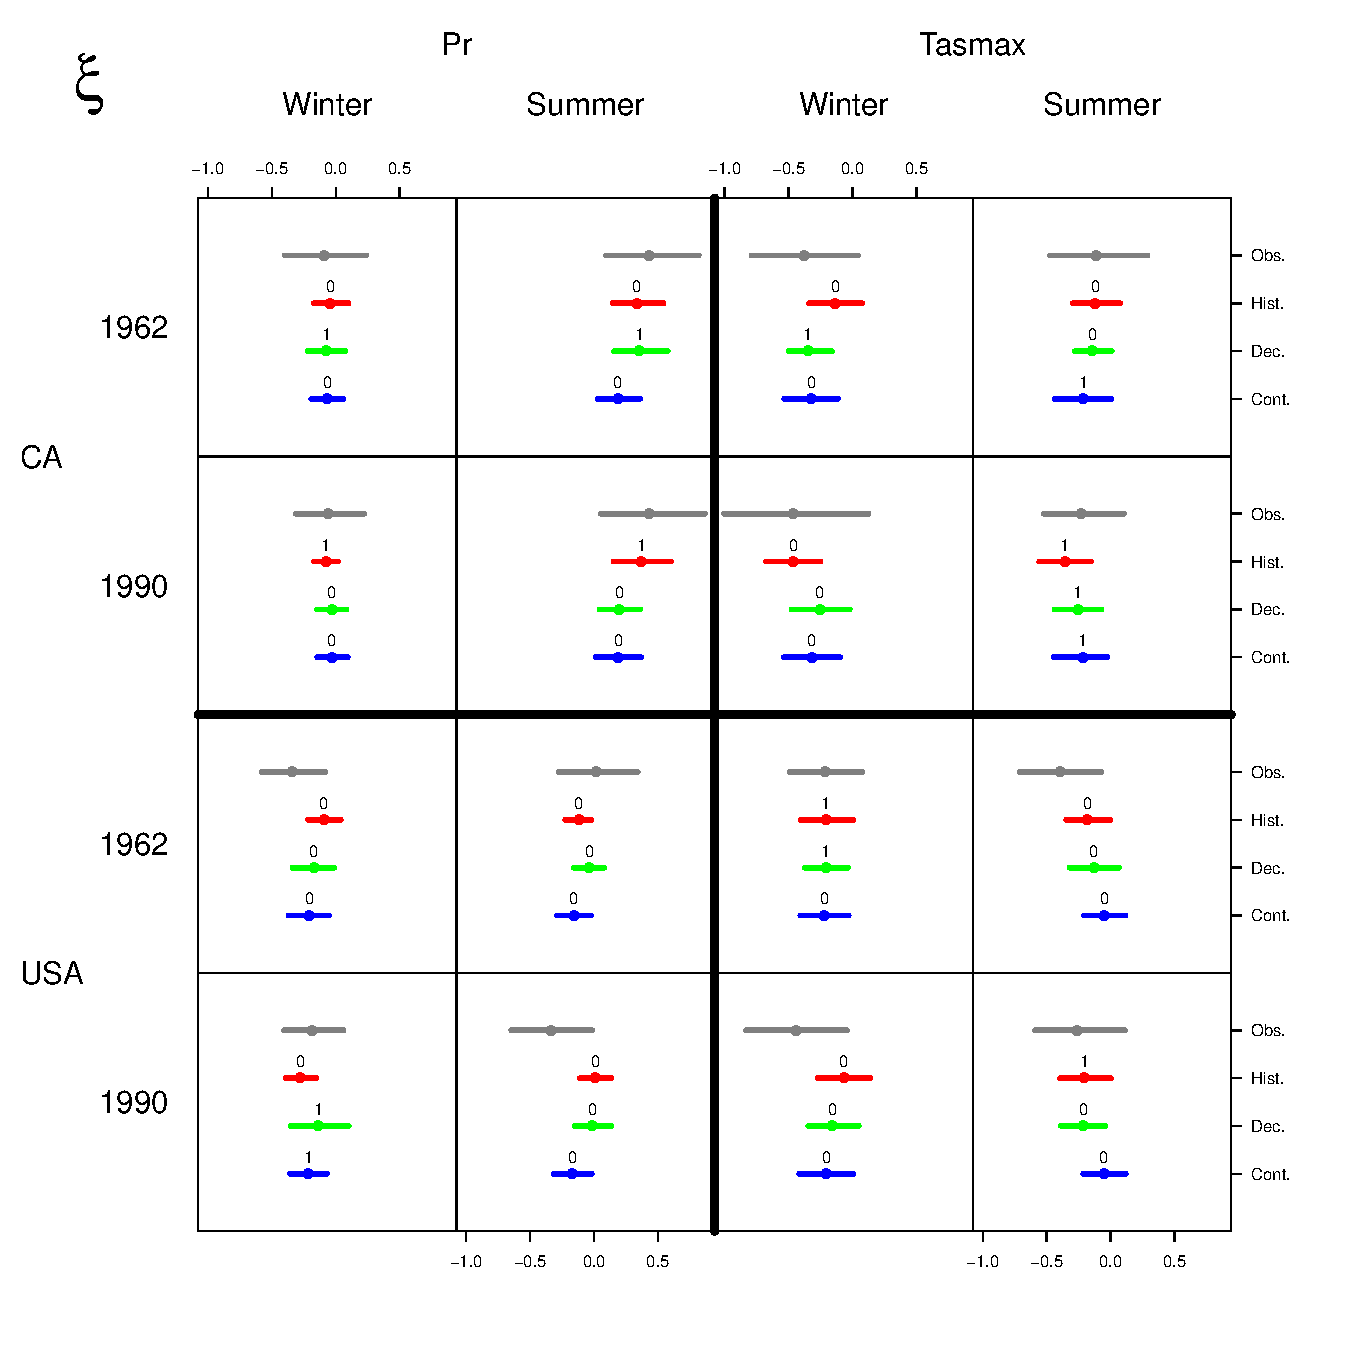
\includegraphics[scale=0.64]{figs/shape.pdf}   % MS (max for margins, but looks offset)
 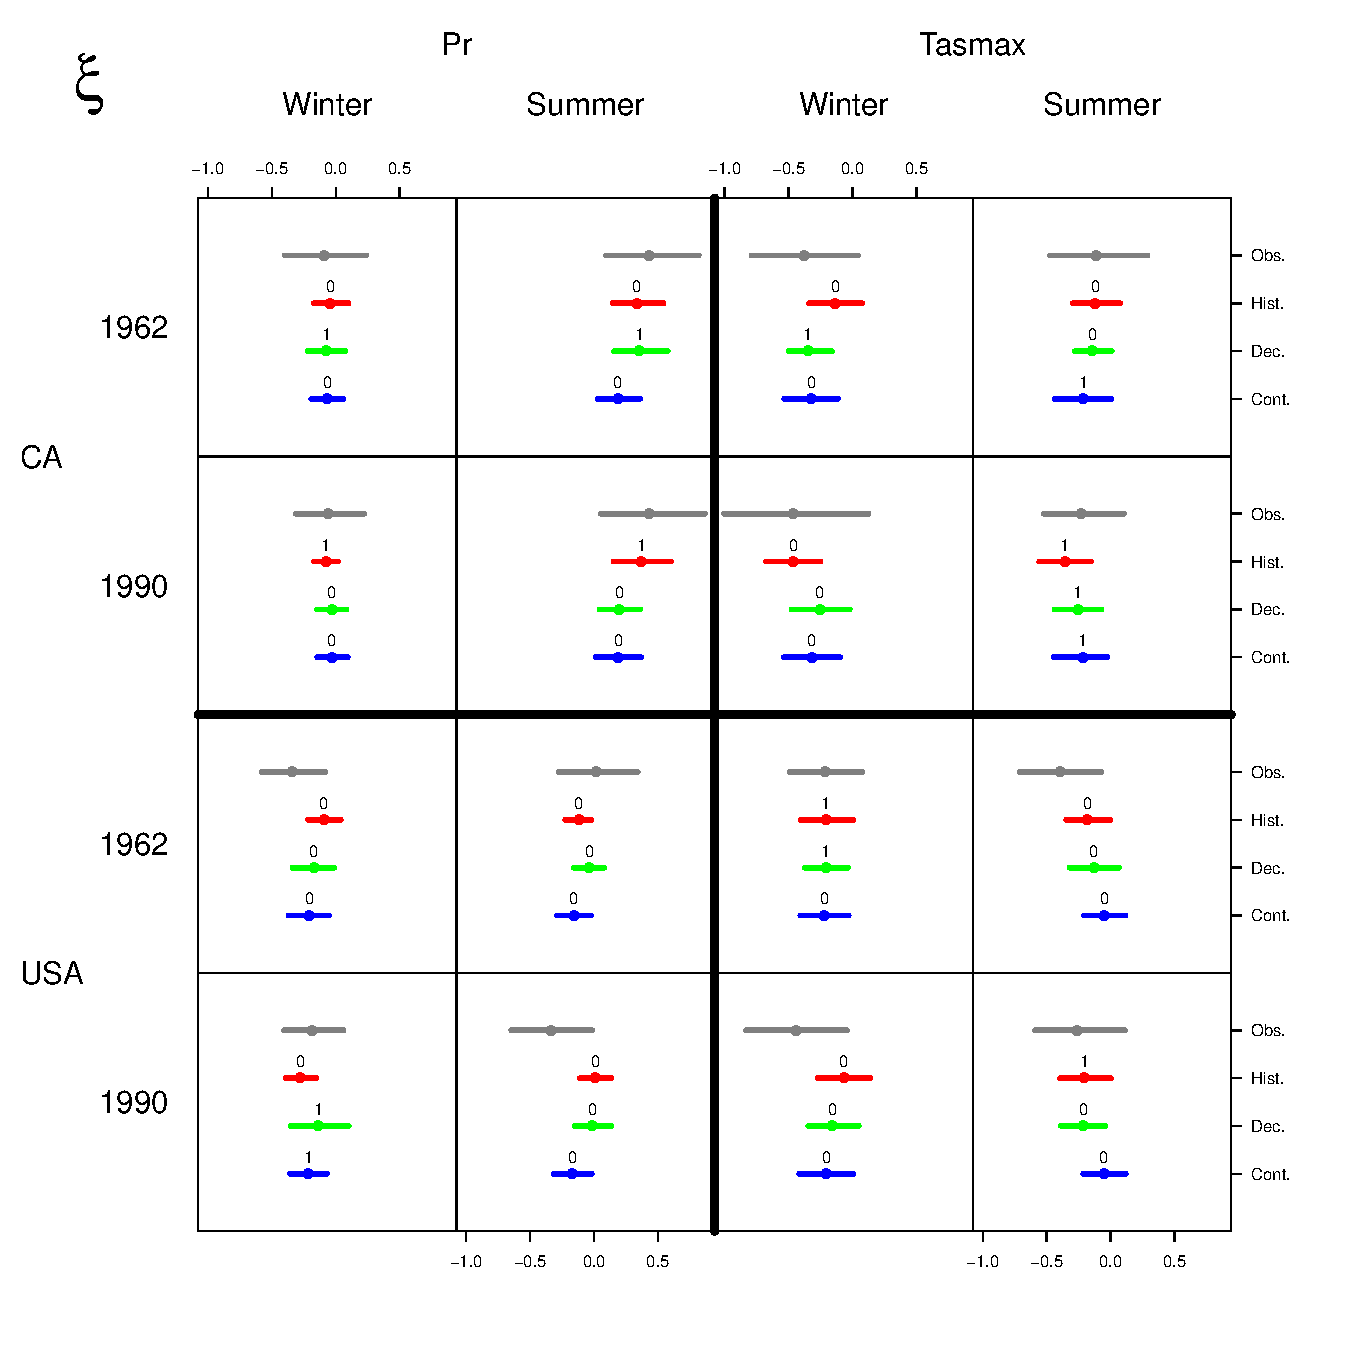
\includegraphics[scale=0.61]{figs/shape.pdf}   % MS (max for no overfull)
%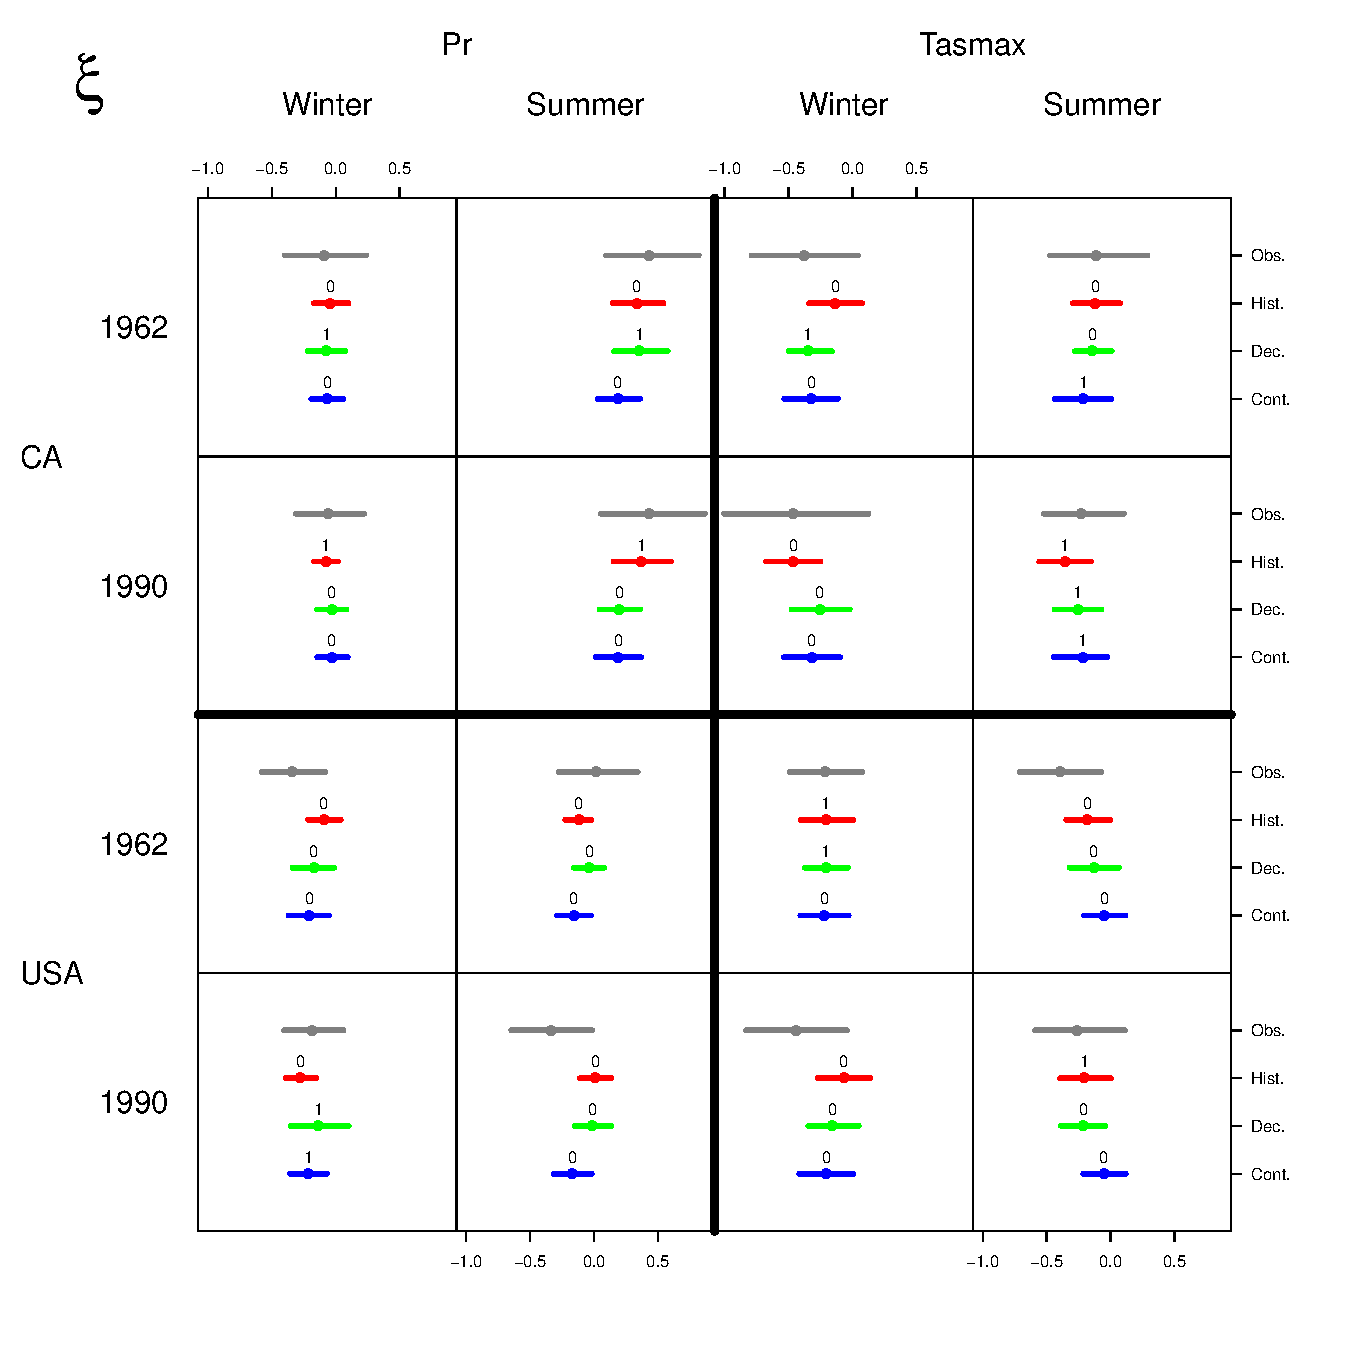
\includegraphics[scale=0.72]{figs/shape.pdf}   % paper
%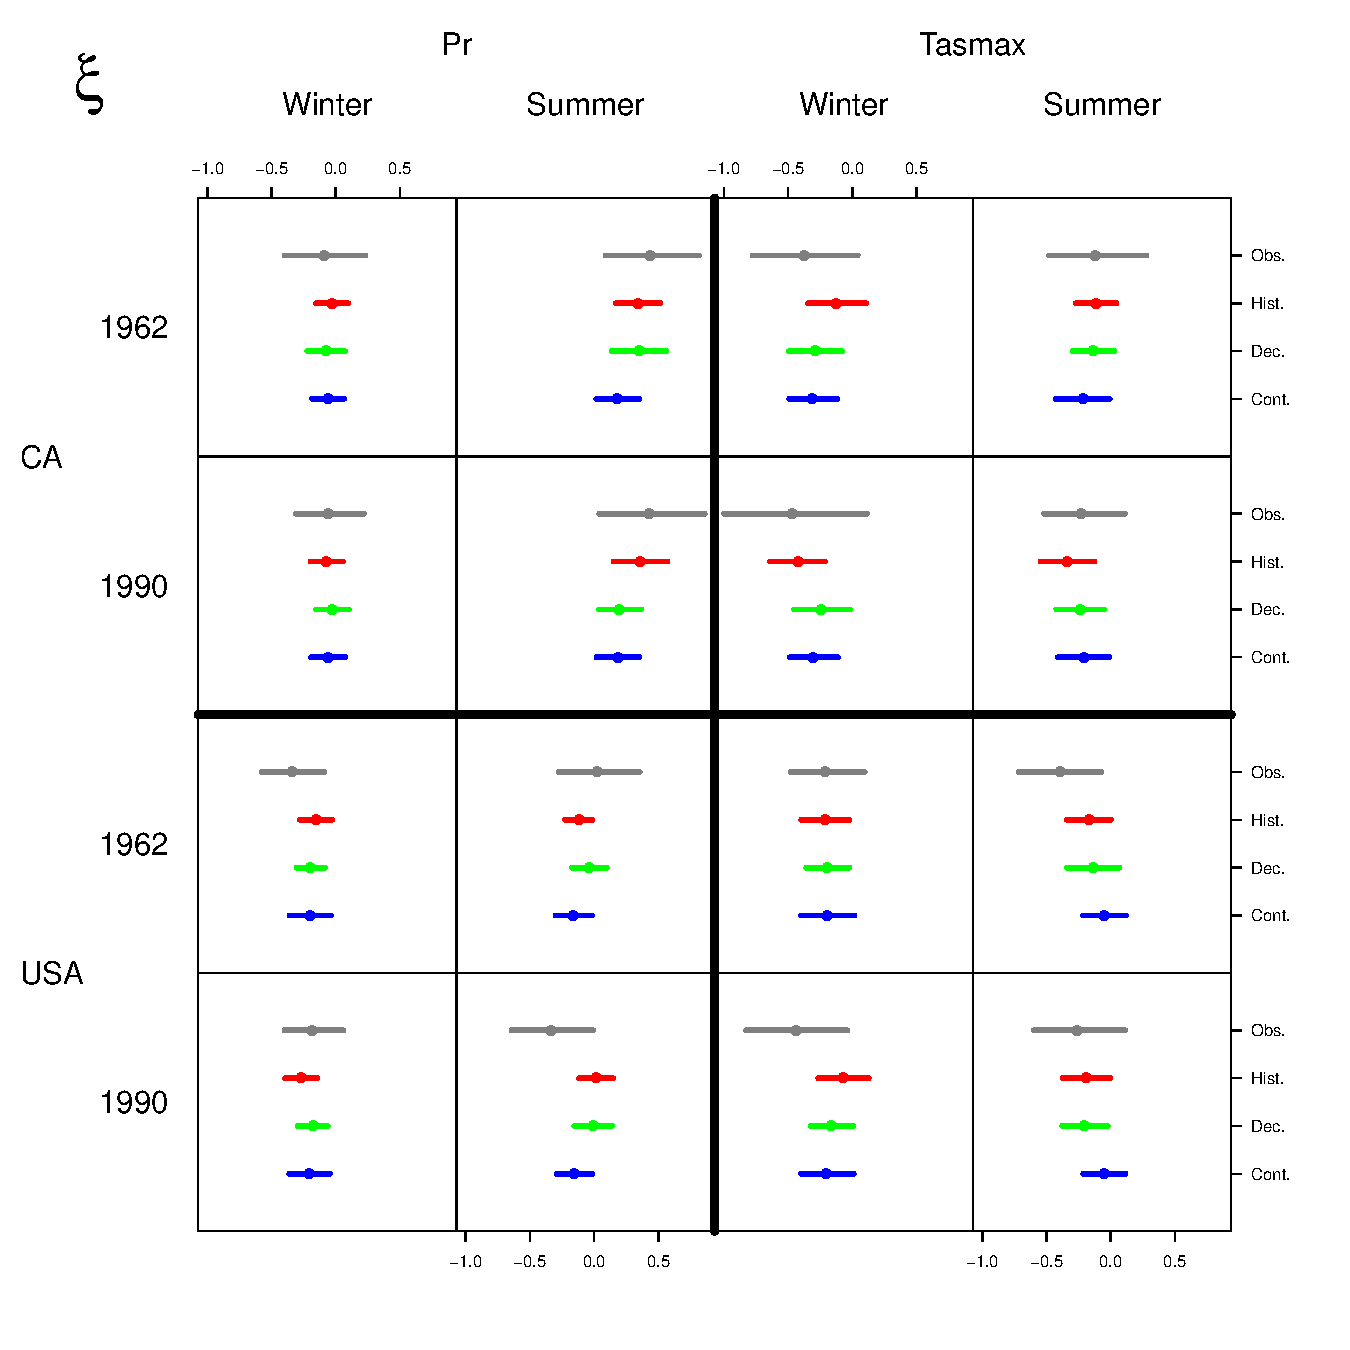
\includegraphics[scale=0.72]{figs/shape_nb.pdf}
\end{center}
%\caption{Posterior shape parameter, $\xi$, under each domain and each of the four data types. The points are the means and the lines mark the 95\% h.p.d. intervals. The number above each point marks whether the observations are similar (in the sense of Bhattacharyya distance) to the replicates of that climate model type---1 means similar, 0 mean not similar. Note: The $x$-axes are the same for every plot. The $y$-axes (for this and all subsequent figures) denote only the data type and thus hold no quantitative meaning.}
\caption{Posterior shape parameter, $\xi$, under each domain and each of the four data types. The points are the means and the lines mark the 95\% h.p.d. intervals. Note: The $x$-axes are the same for every plot. The $y$-axes (for this and all subsequent figures) denote only the data type and thus hold no quantitative meaning.}
\label{ksi}
\end{figure}

\begin{figure}
\begin{center}
 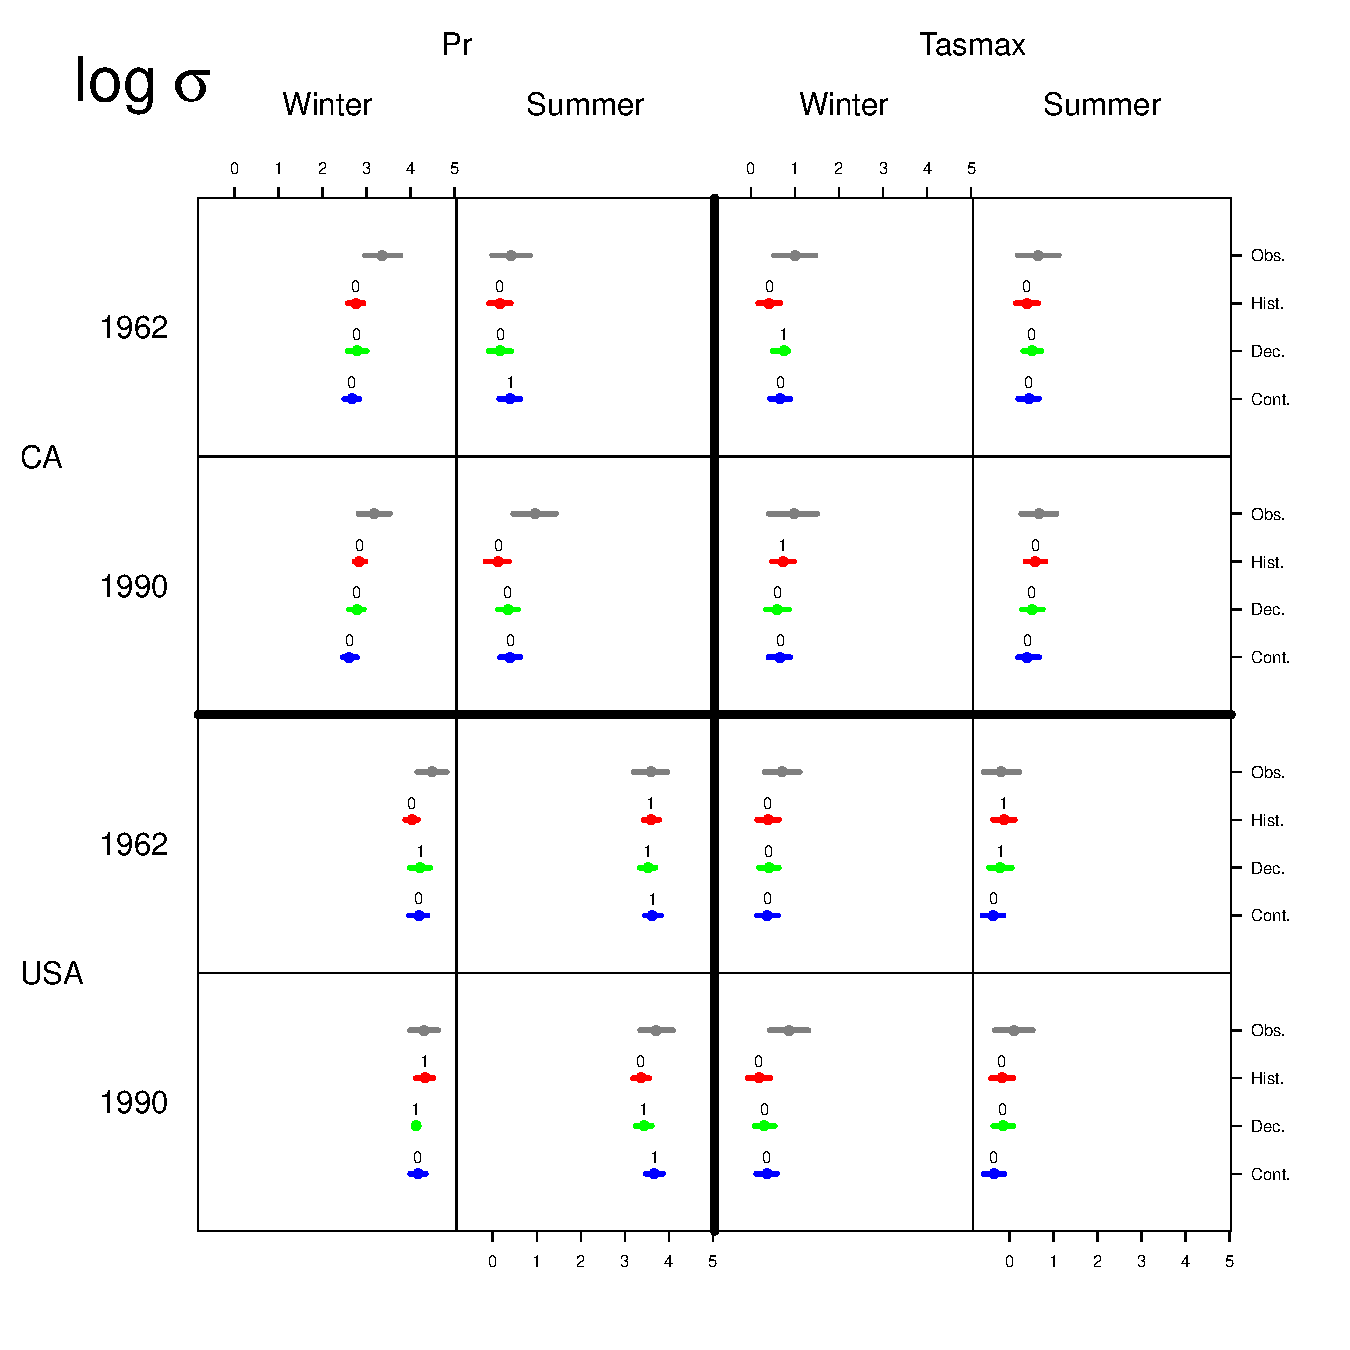
\includegraphics[scale=0.61]{figs/log_sigma.pdf}
%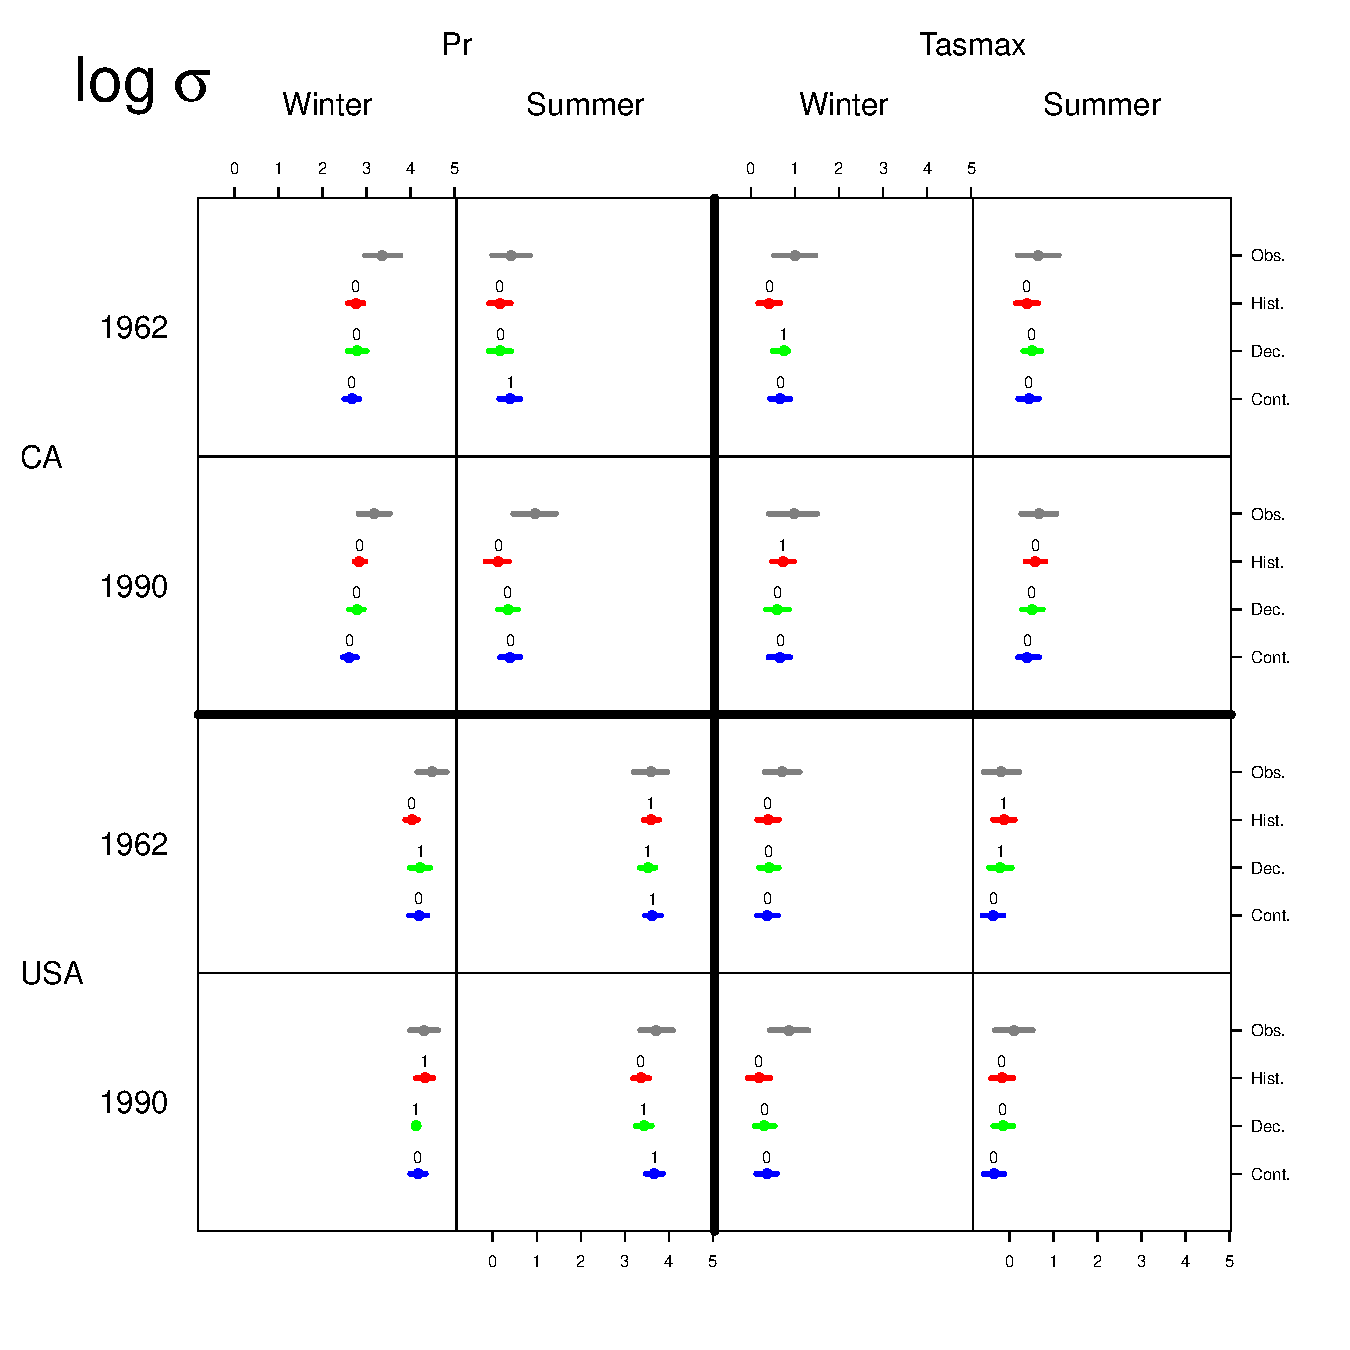
\includegraphics[scale=0.72]{figs/log_sigma.pdf}
%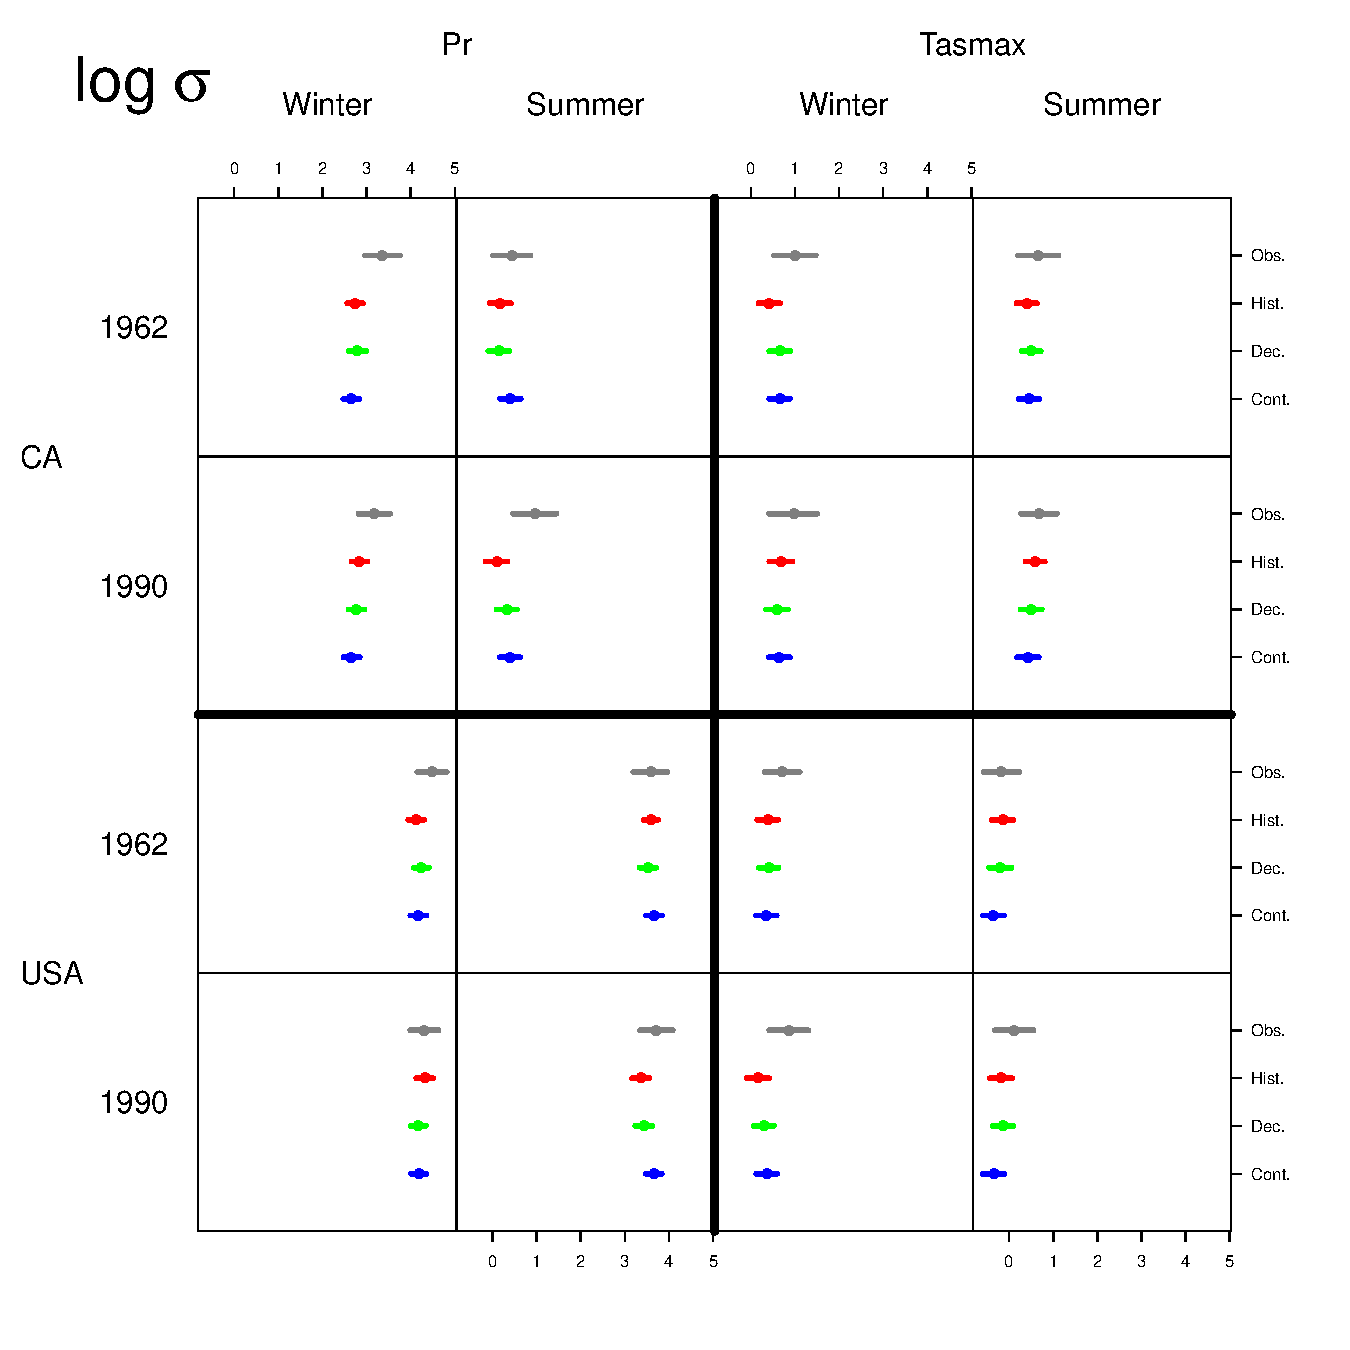
\includegraphics[scale=0.72]{figs/log_sigma_nb.pdf}
\end{center}
\caption{Natural logarithm of the posterior scale. For the CanCM4 simulations, the parameter shown is $\log (\alpha/\beta)$ (the mean scale) because $\sigma_i$ follows a Gamma distribution with mean $\alpha/\beta$. No change of variables is necessary for the observations. Note: The $x$-axes are the same for every plot.}
\label{sigma}
\end{figure}

\begin{figure}
\begin{center}
 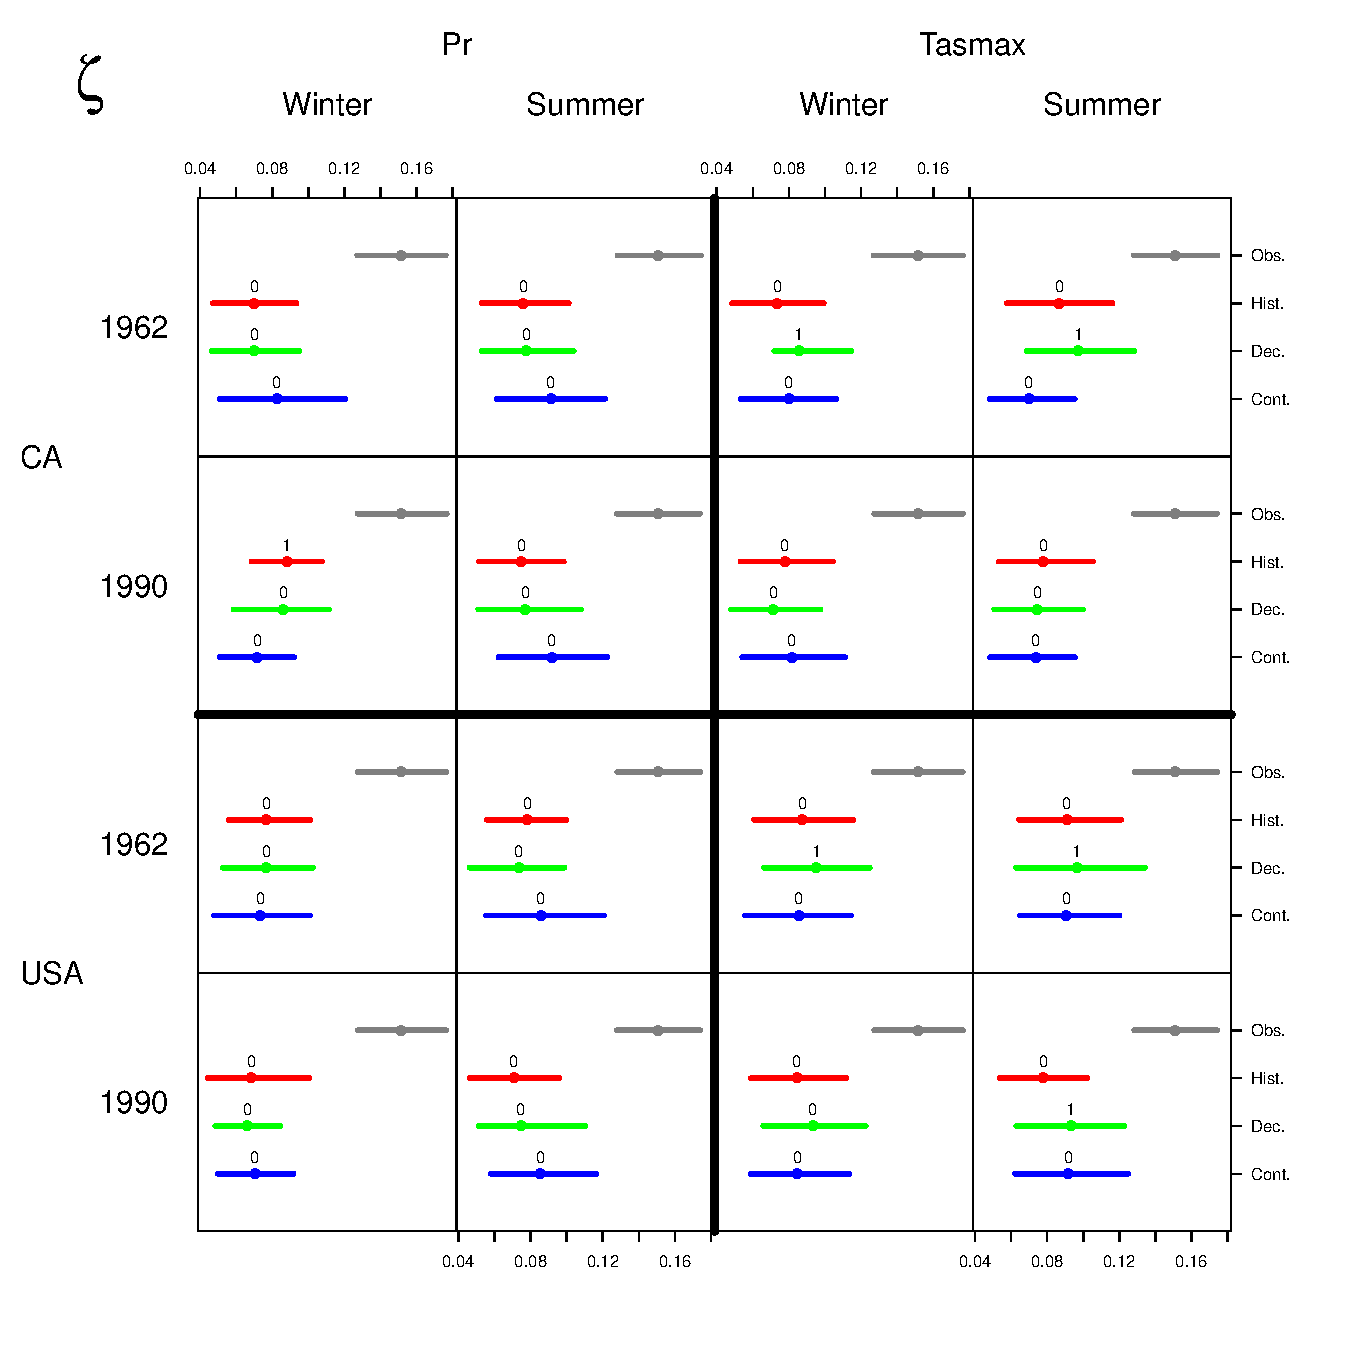
\includegraphics[scale=0.61]{figs/zeta.pdf}
%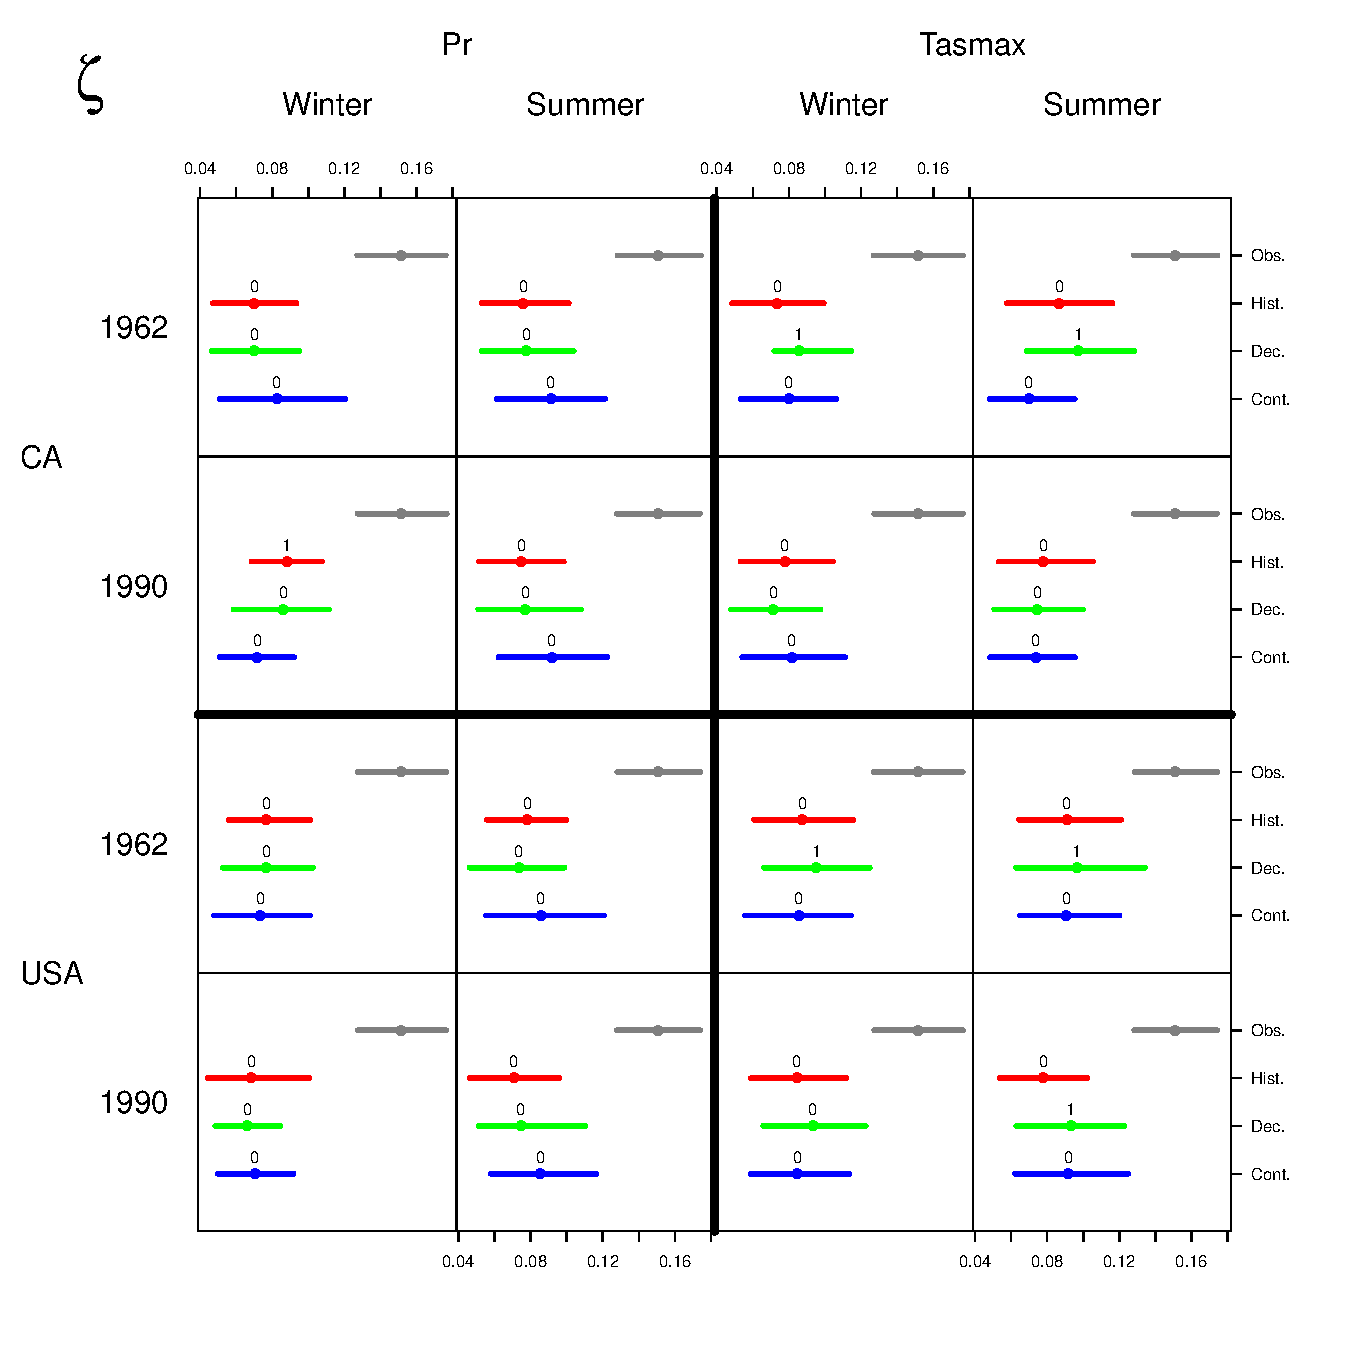
\includegraphics[scale=0.72]{figs/zeta.pdf}
%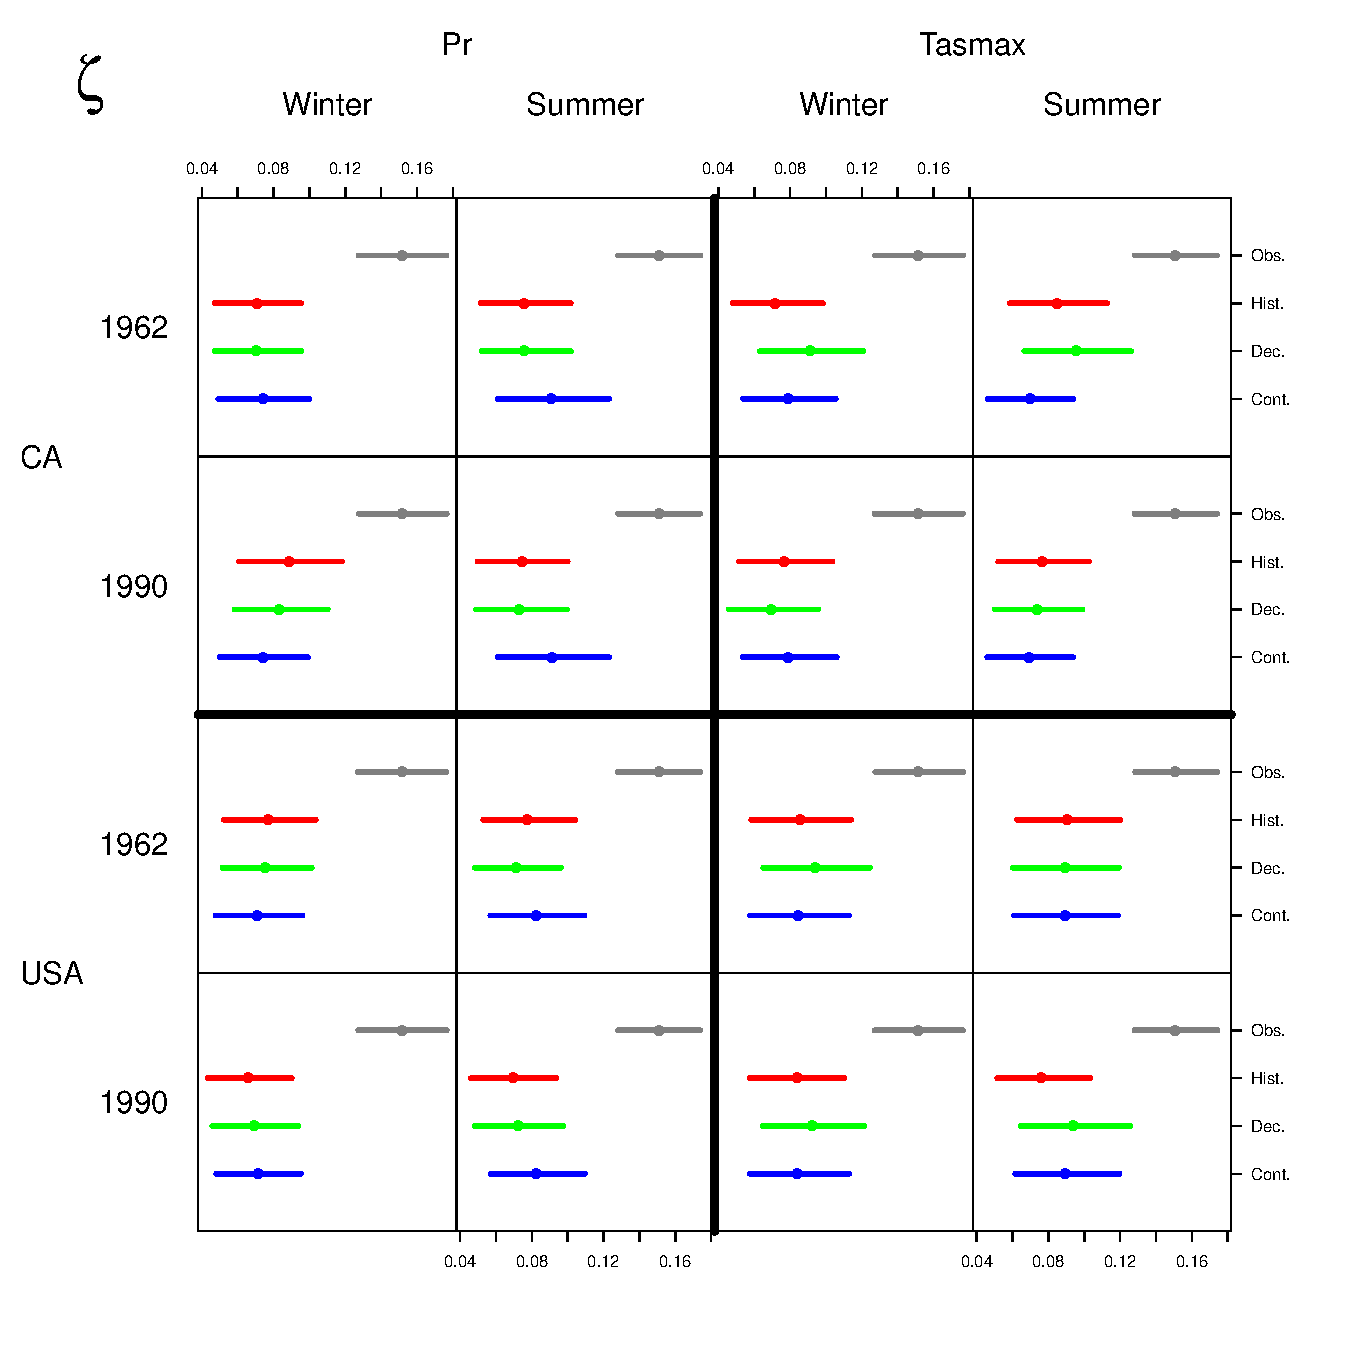
\includegraphics[scale=0.72]{figs/zeta_nb.pdf}
\end{center}
\caption{The probability of exceeding the threshold. These parameters are closely tied to the threshold, a user-specified quantity. Since we chose thresholds as the $0.95$ quantile for the climate simulations and the $0.85$ quantile for the observations, we do not expect there to be much overlap between these posteriors.}
\label{zeta}
\end{figure}

\begin{figure}
\begin{center}
 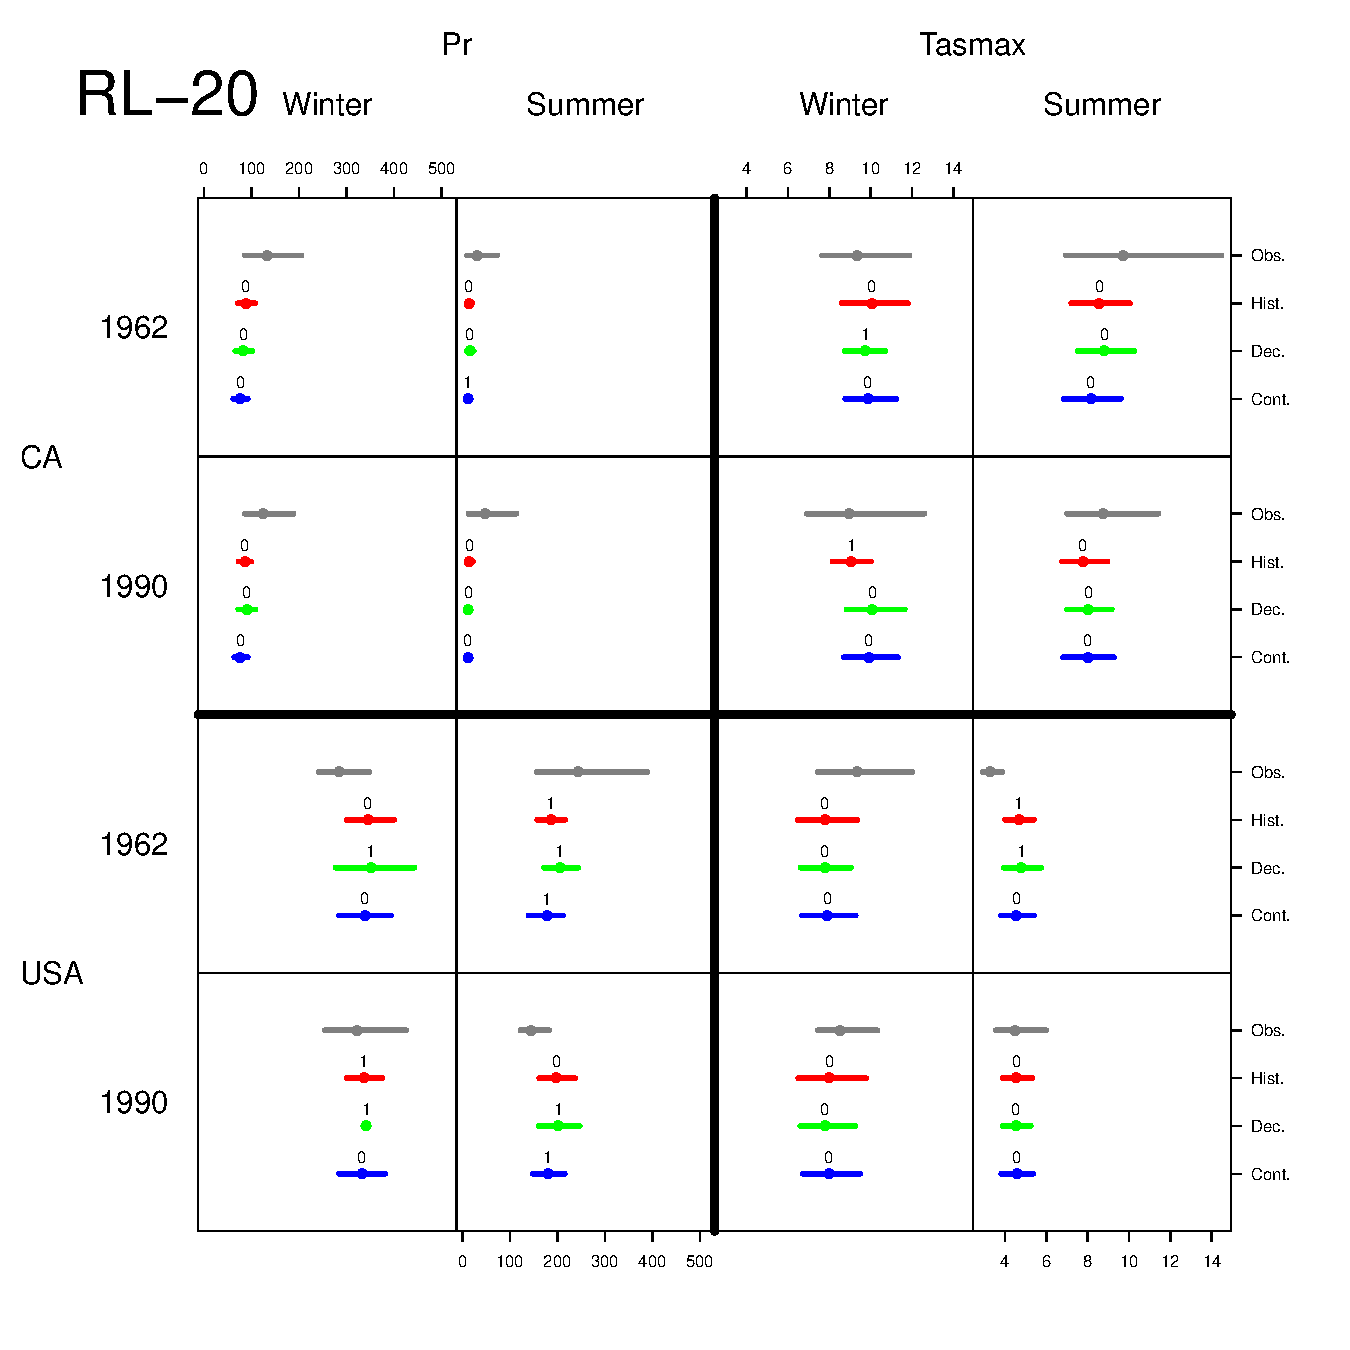
\includegraphics[scale=0.61]{figs/rl20.pdf}
%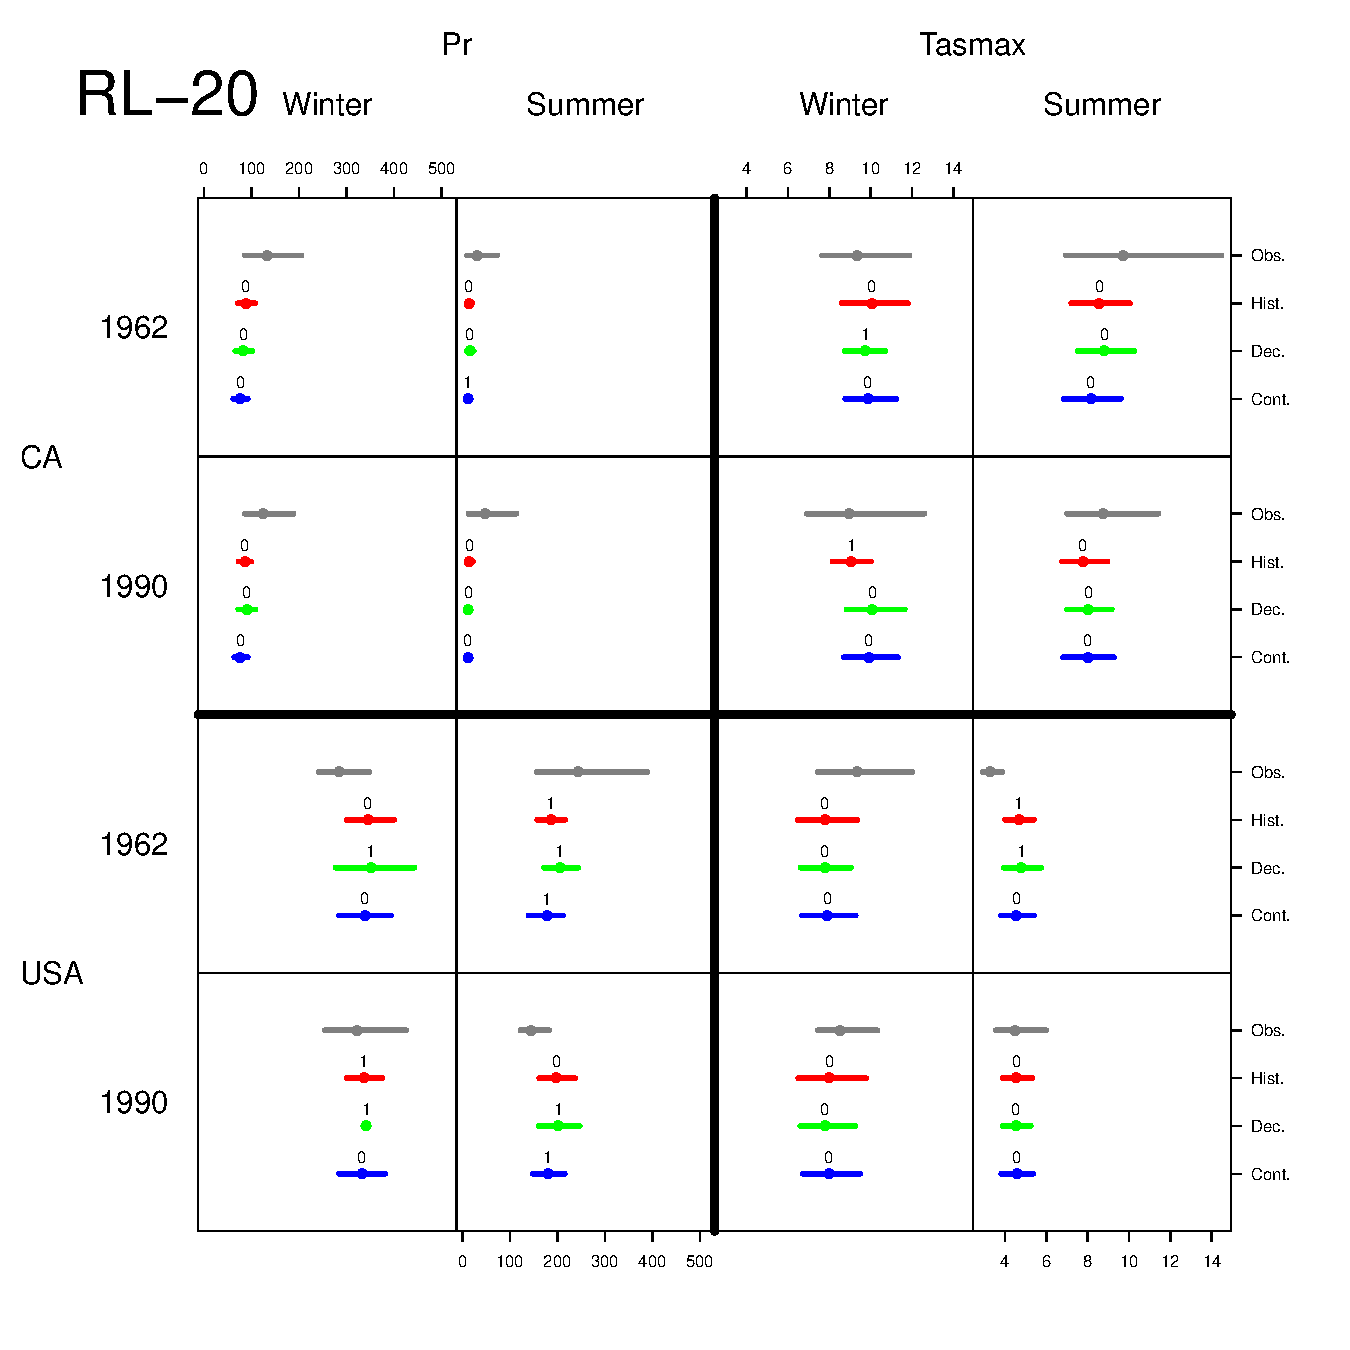
\includegraphics[scale=0.72]{figs/rl20.pdf}
%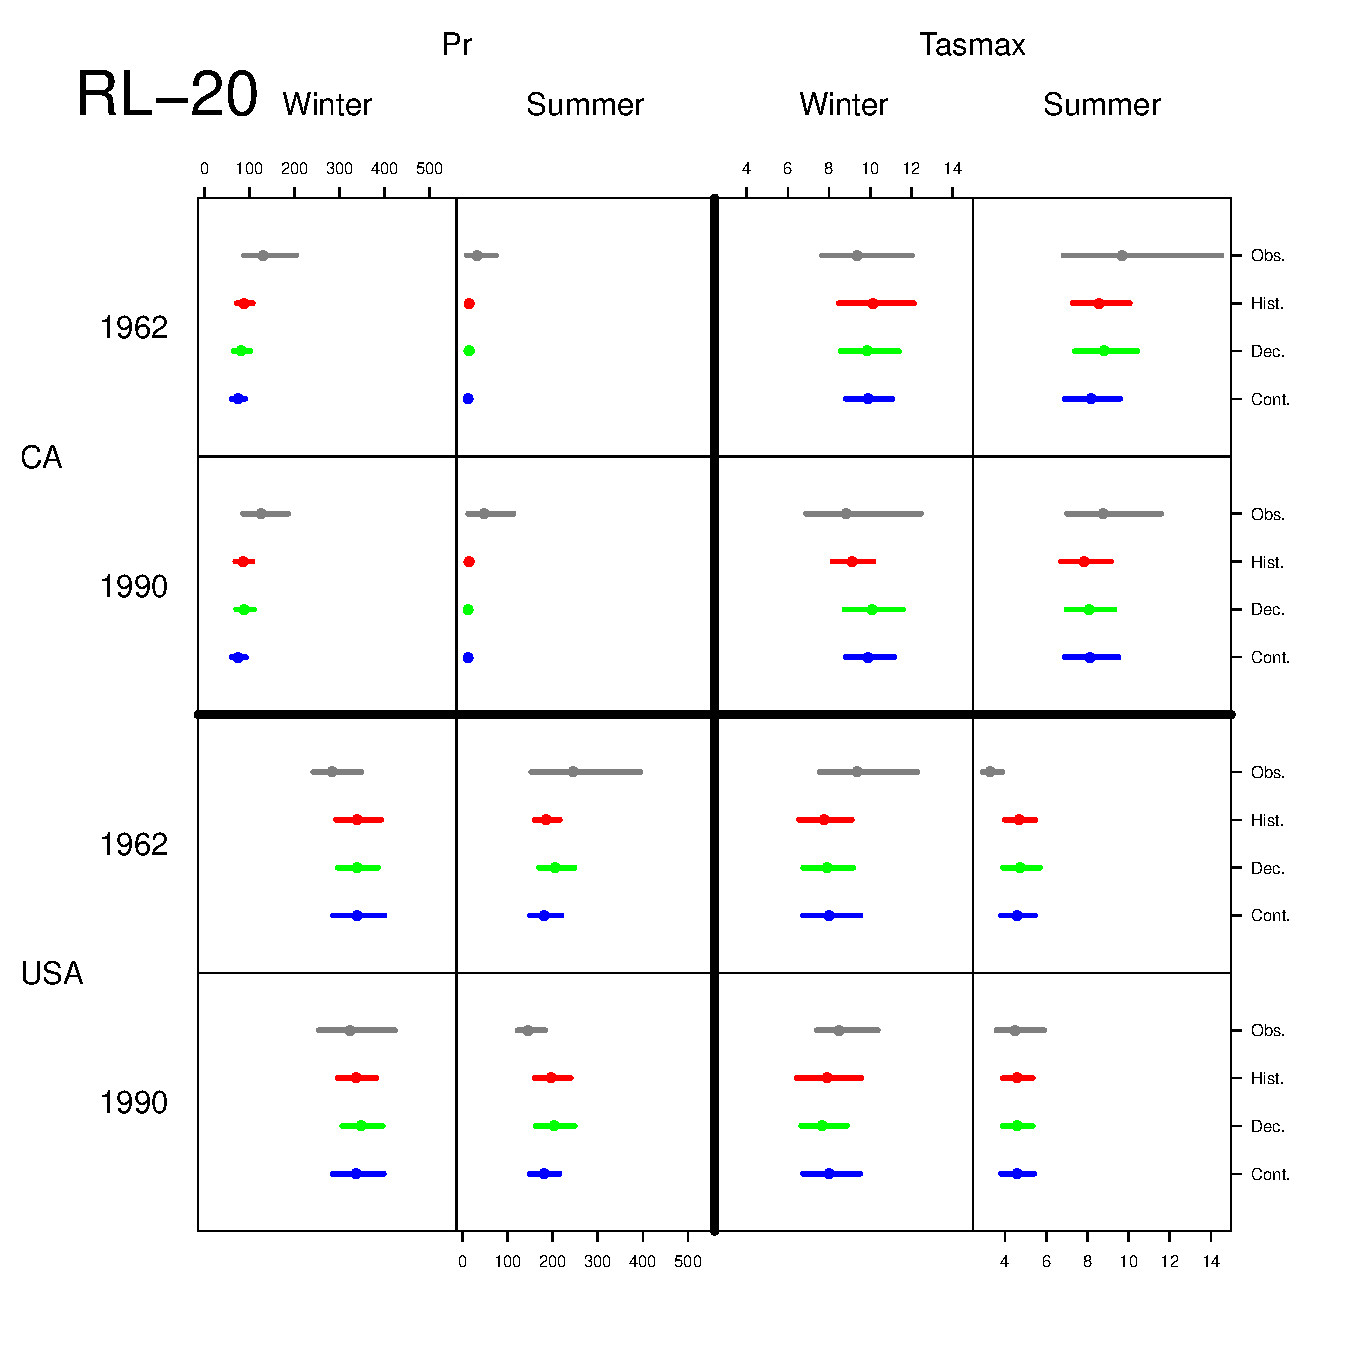
\includegraphics[scale=0.72]{figs/rl20_nb.pdf}
\end{center}
\caption{20-year return levels. Note: The left two columns have the same $x$-axes, which are different than those in the right two columns, which have the same.}
\label{20rl}
\end{figure}

\begin{figure}
\begin{center}
 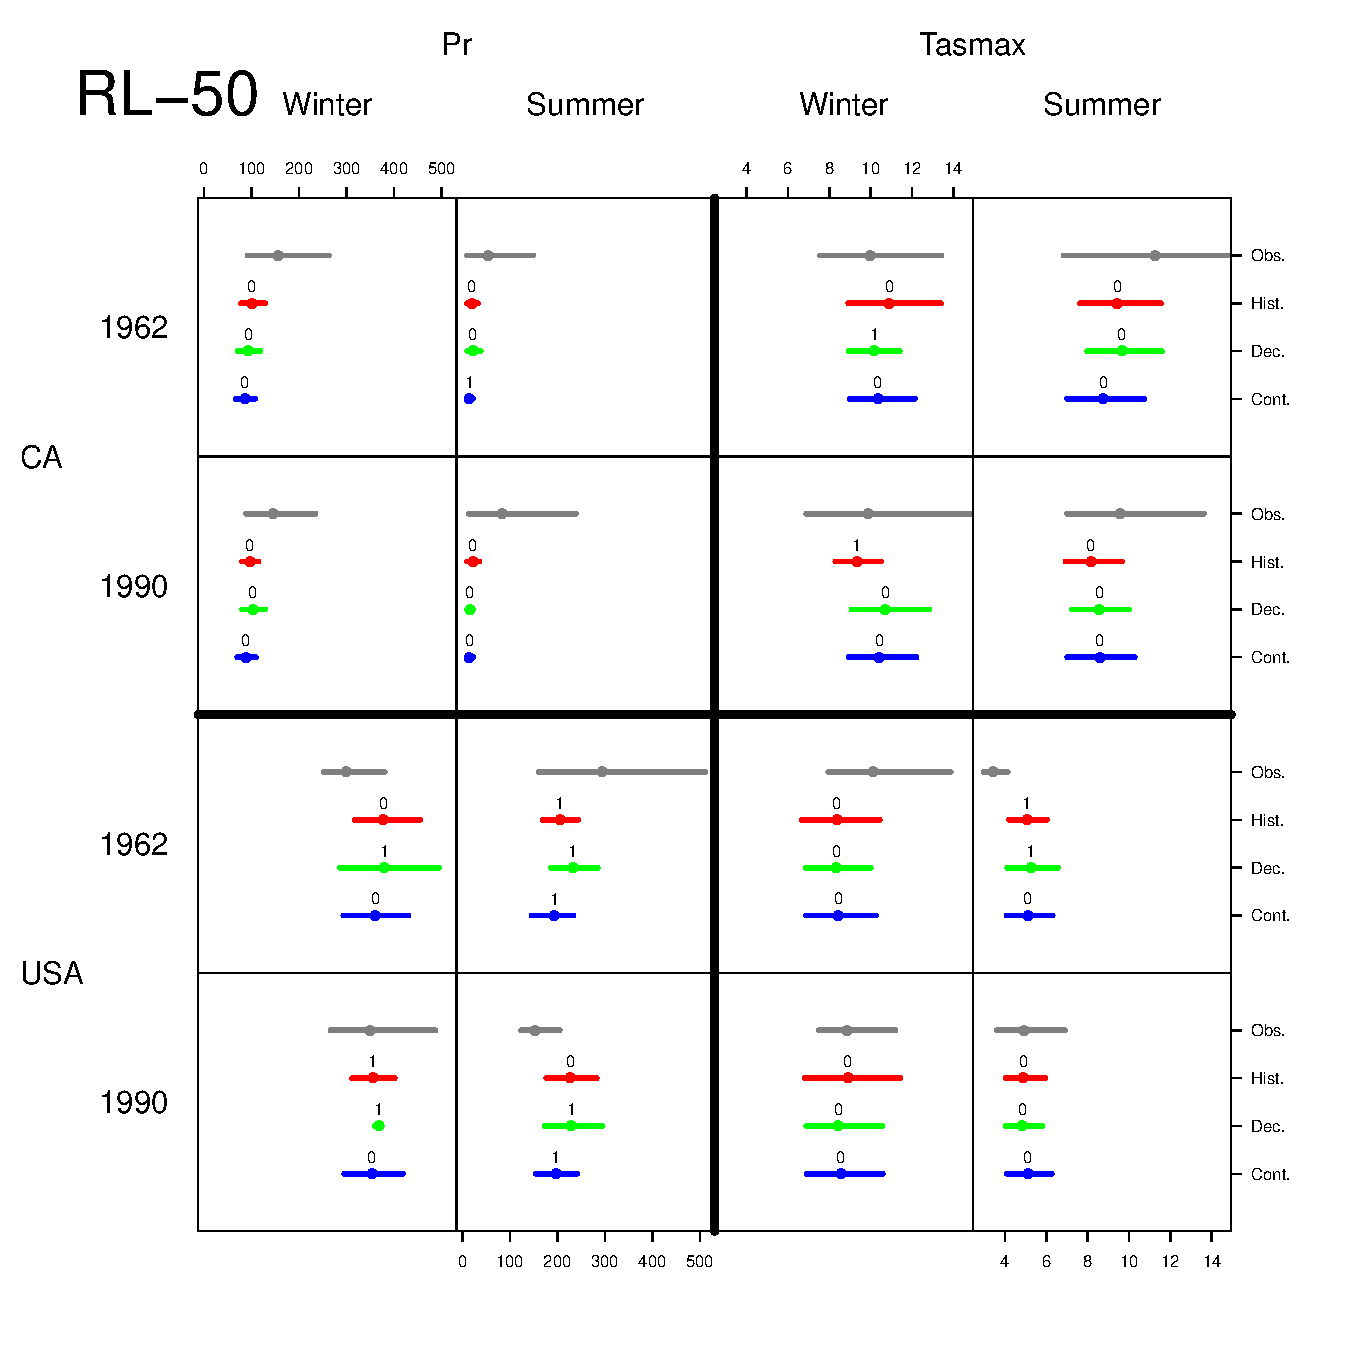
\includegraphics[scale=0.61]{figs/rl50.pdf}
%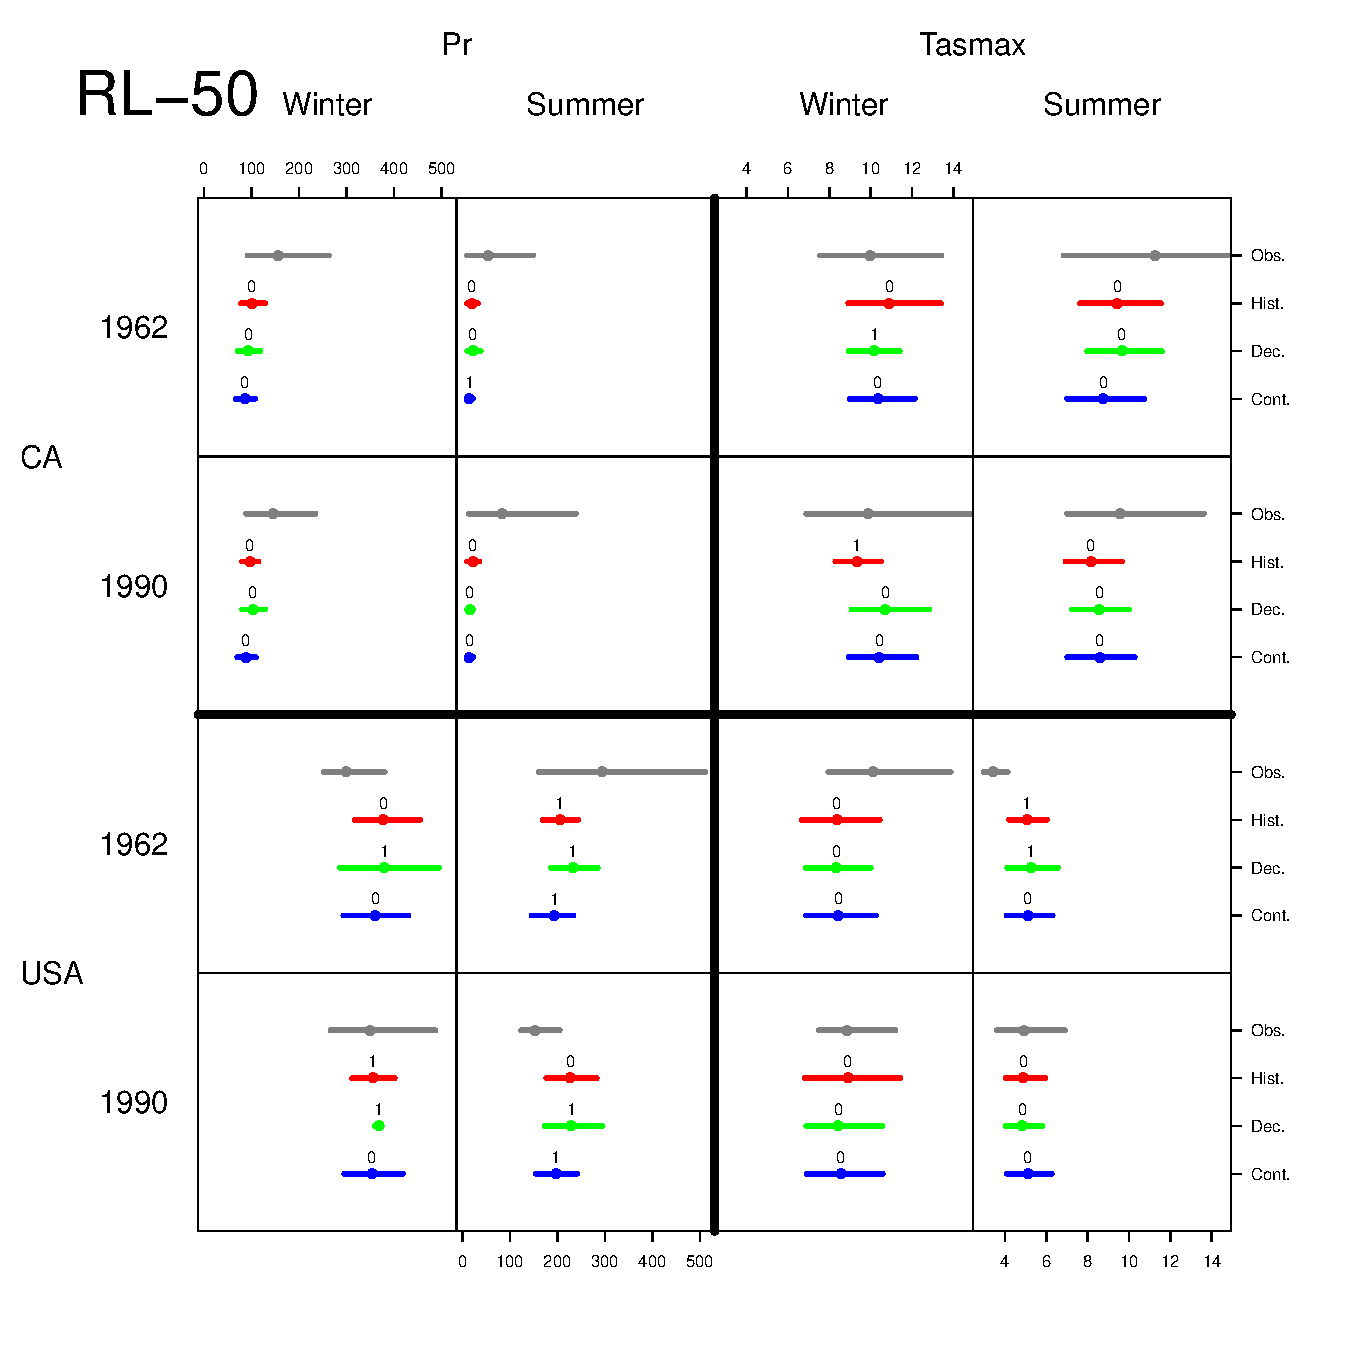
\includegraphics[scale=0.72]{figs/rl50.pdf}
%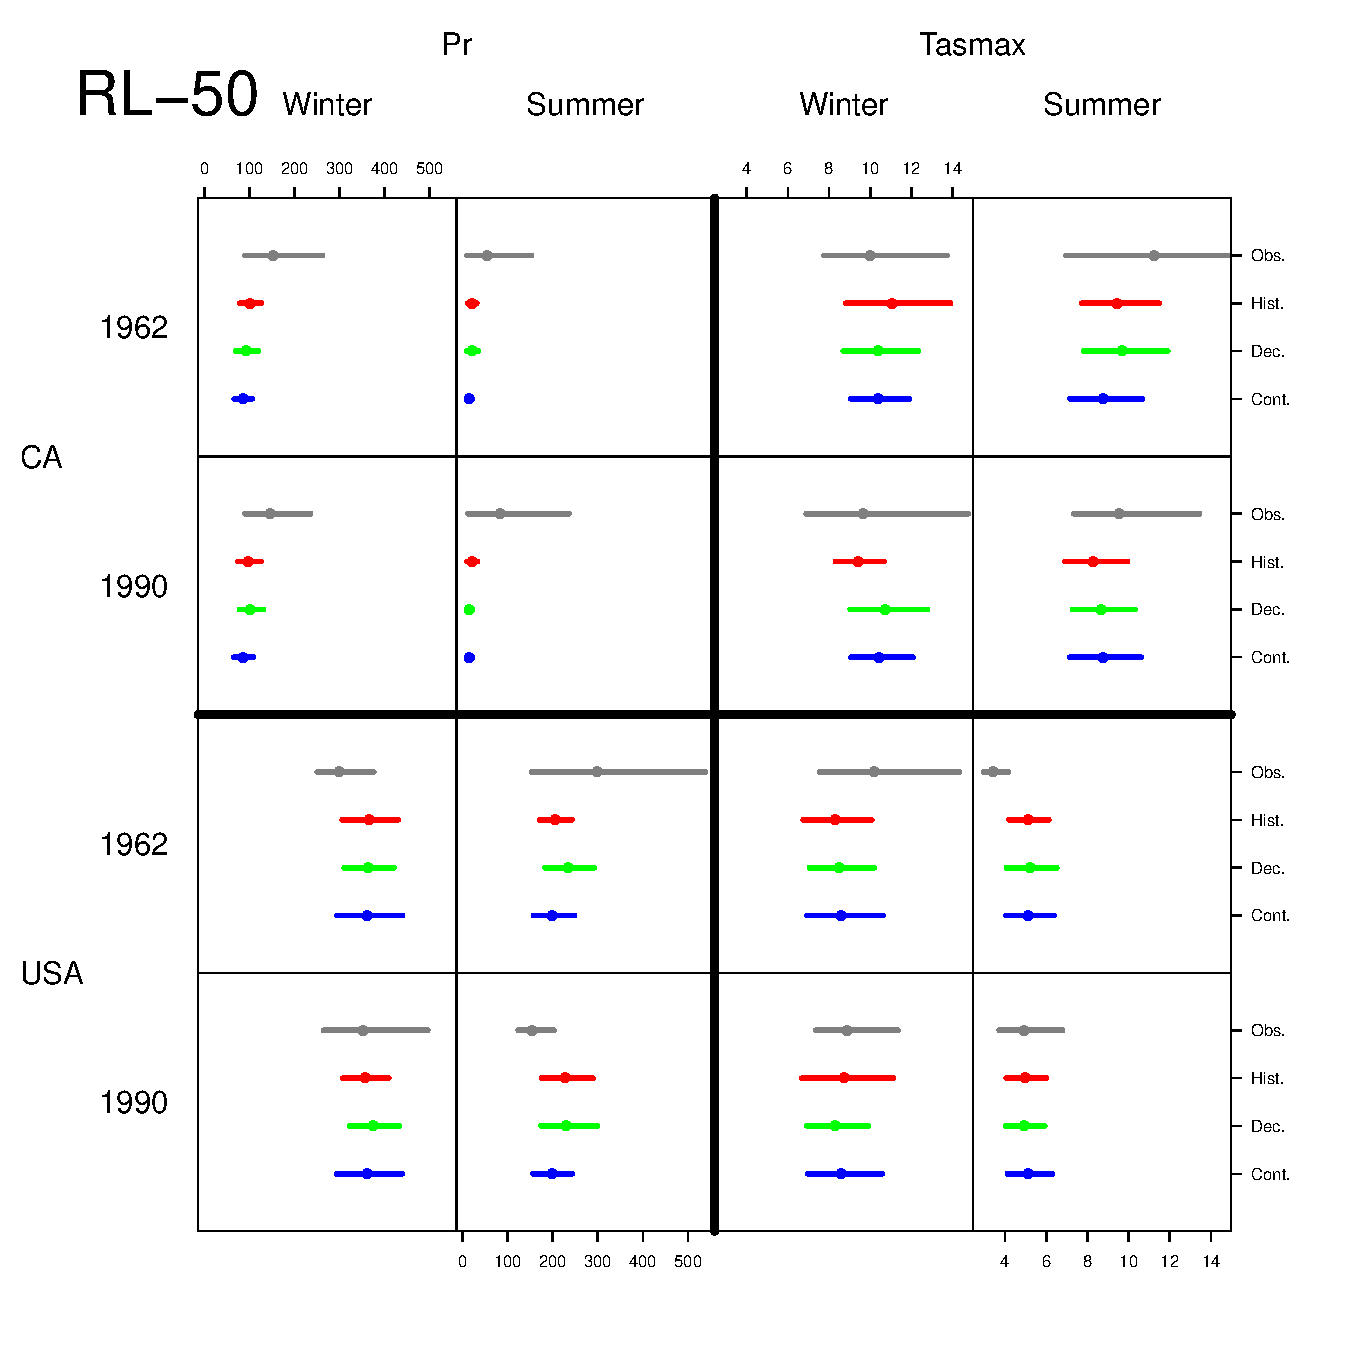
\includegraphics[scale=0.72]{figs/rl50_nb.pdf}
\end{center}
\caption{50-year return levels. The $x$-axes are the same as those in Figure \ref{20rl}.}
\label{50rl}
\end{figure}

\begin{figure}
\begin{center}
 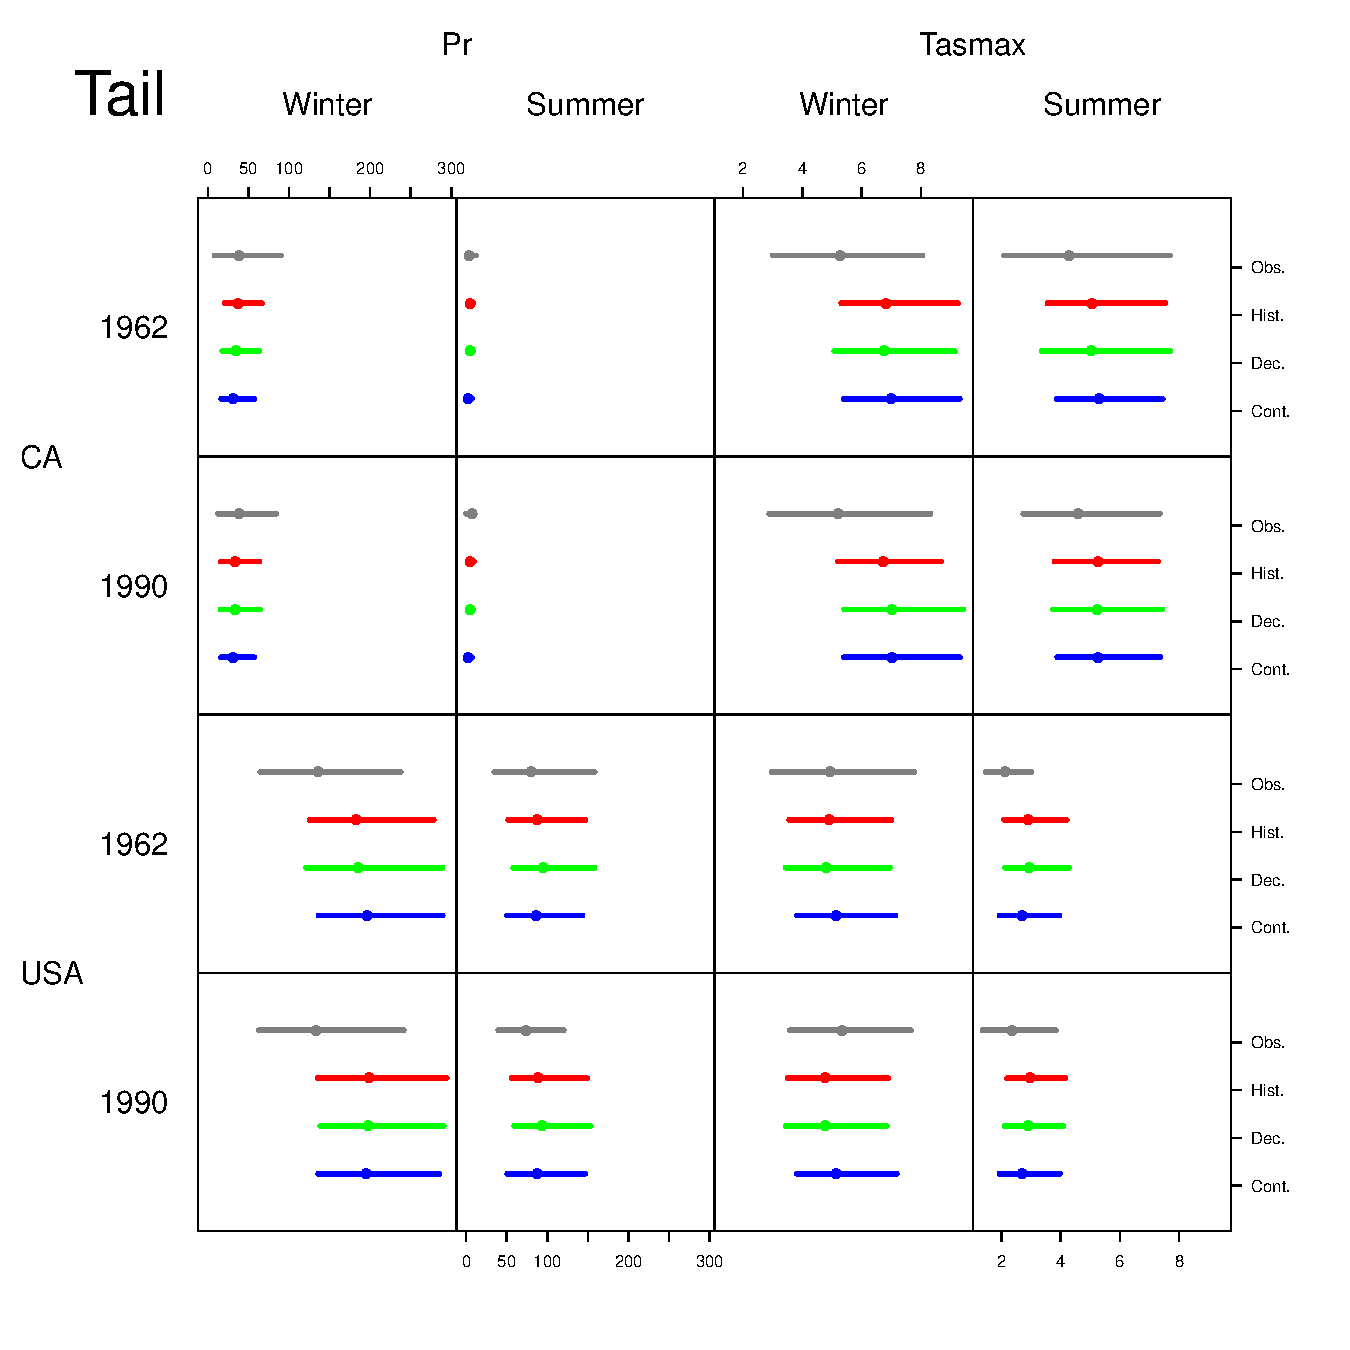
\includegraphics[scale=0.61]{figs/tail.pdf}
%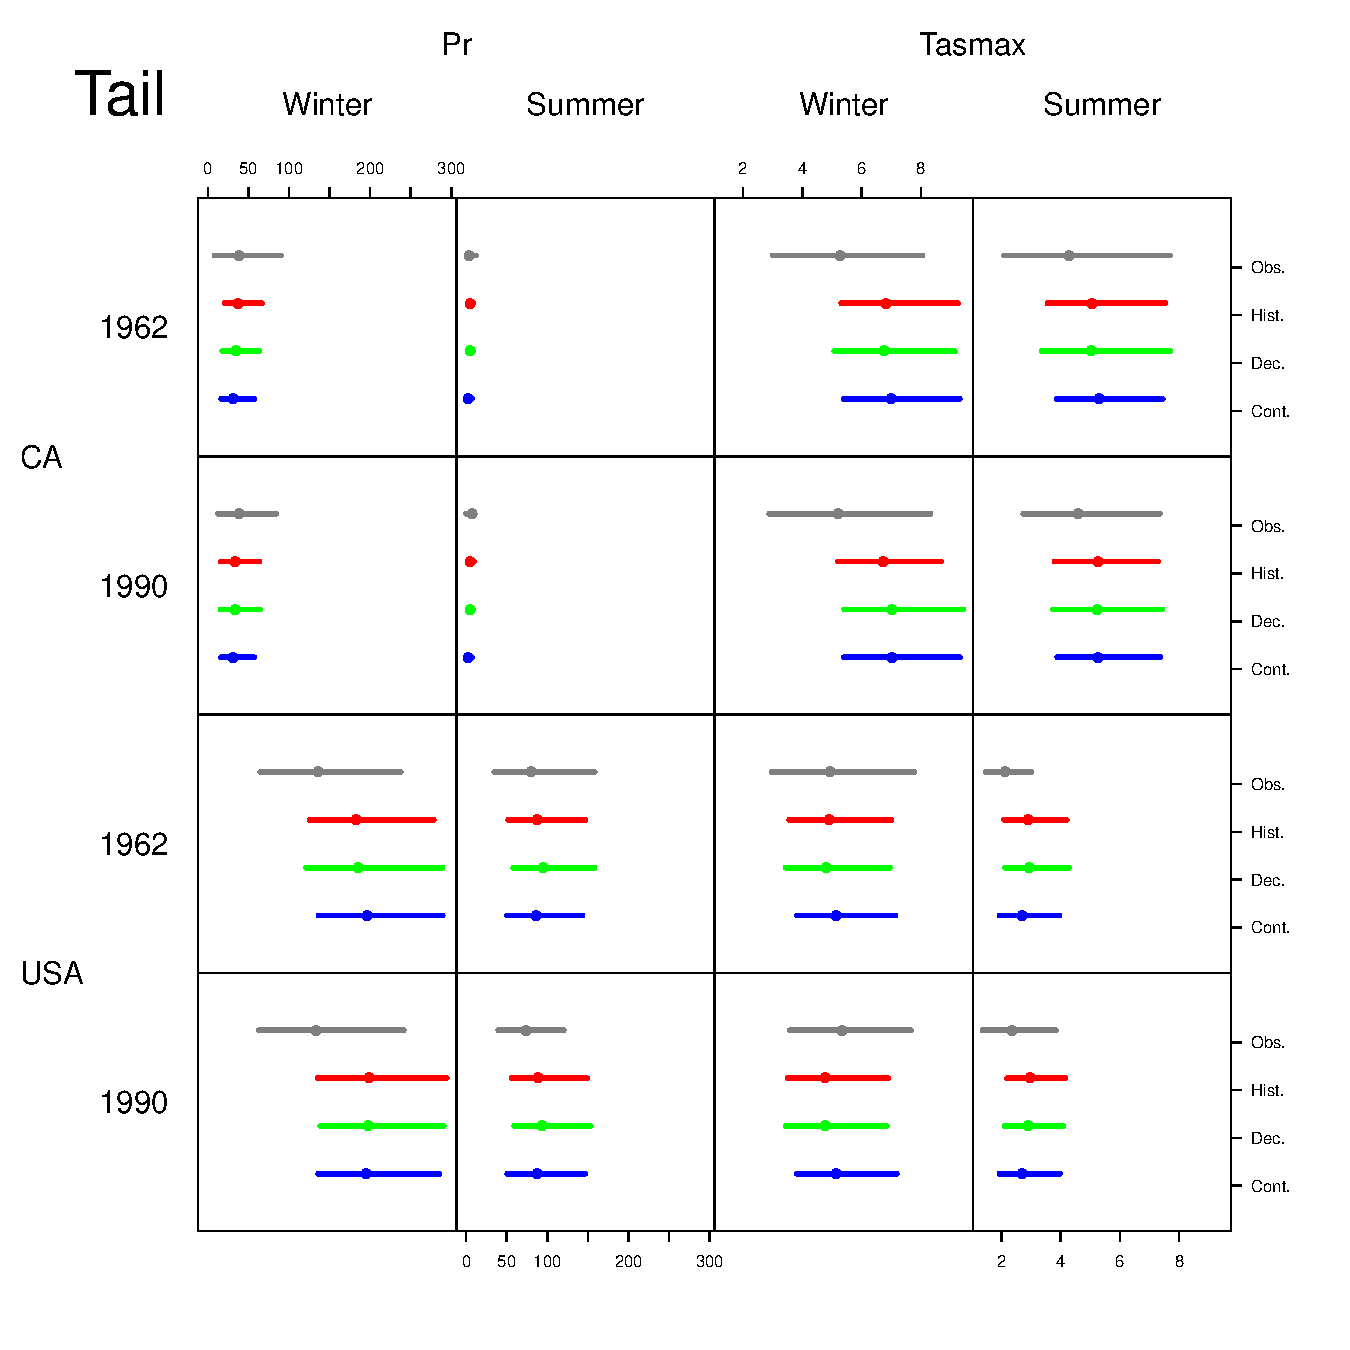
\includegraphics[scale=0.72]{figs/tail.pdf}
%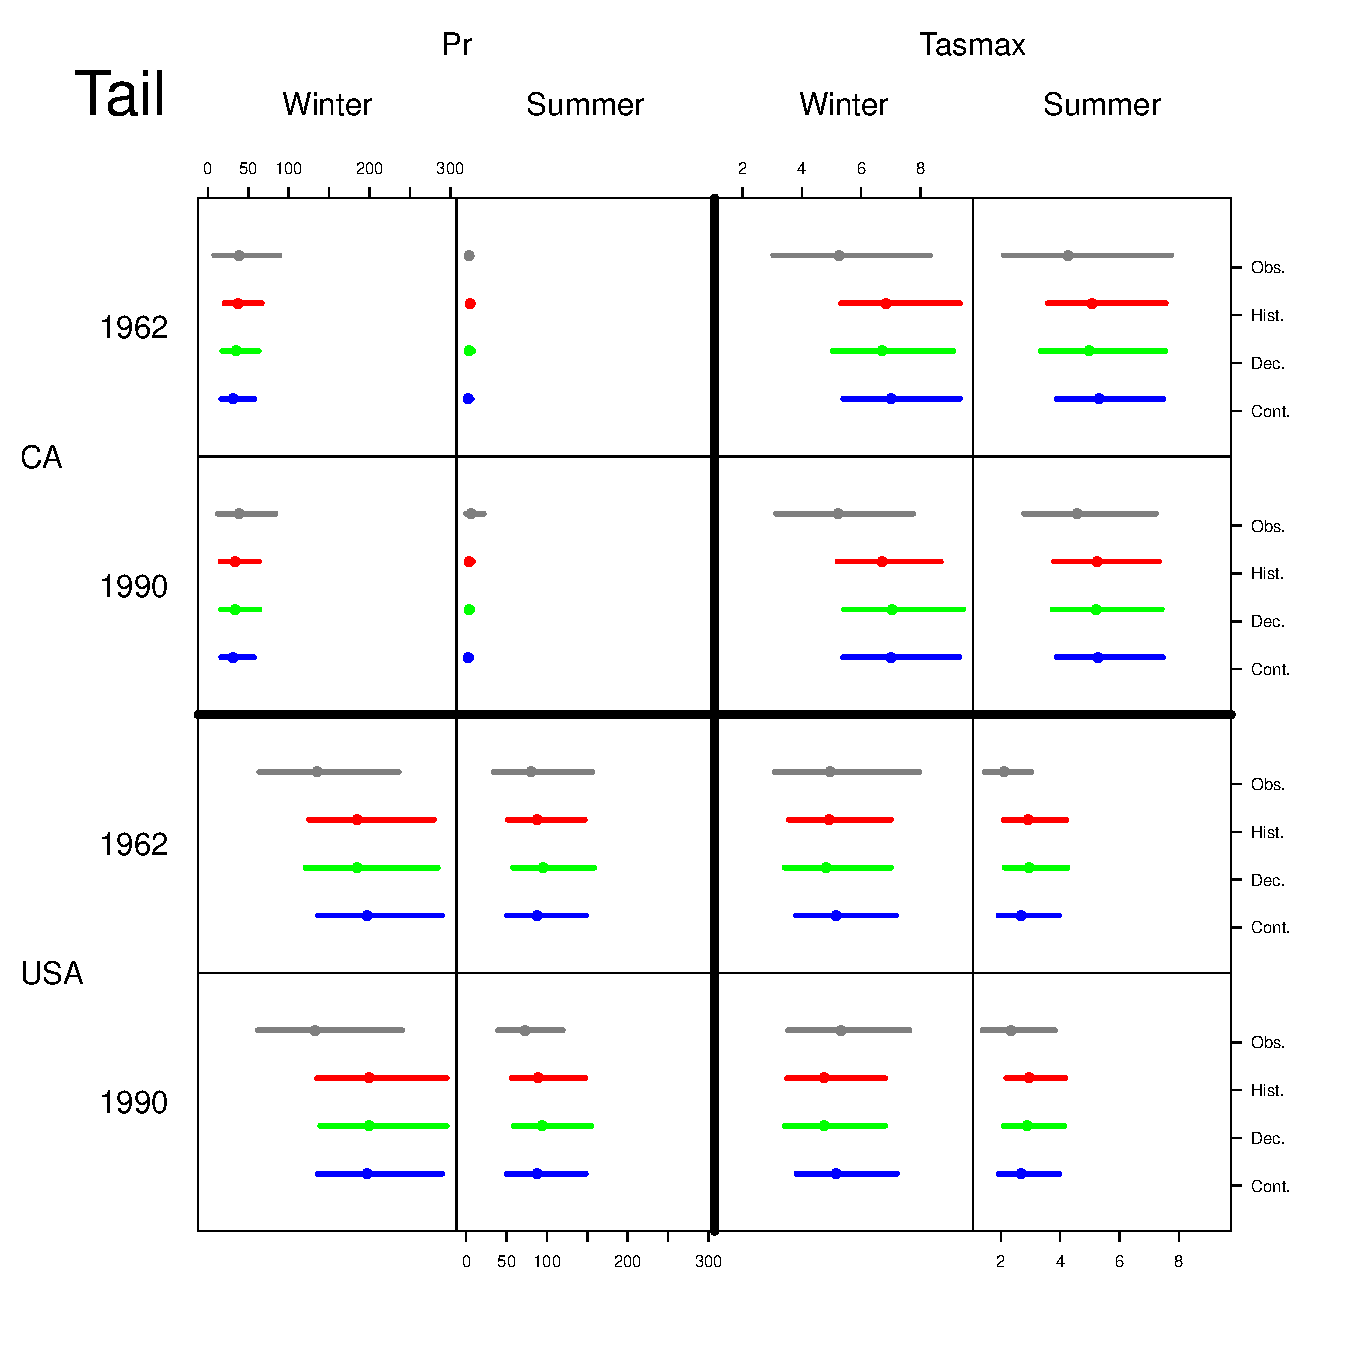
\includegraphics[scale=0.72]{figs/tail_nb.pdf}
\end{center}
\caption{Mean and 95\% h.p.d. for the upper tail (i.e. the generalized Pareto) of the ensemble average. As in Figures \ref{20rl} and \ref{50rl}, the left two columns have the same $x$-axes and the right two columns have the same $x$-axes.}
\label{tail}
\end{figure}

\begin{figure}
\begin{center}
 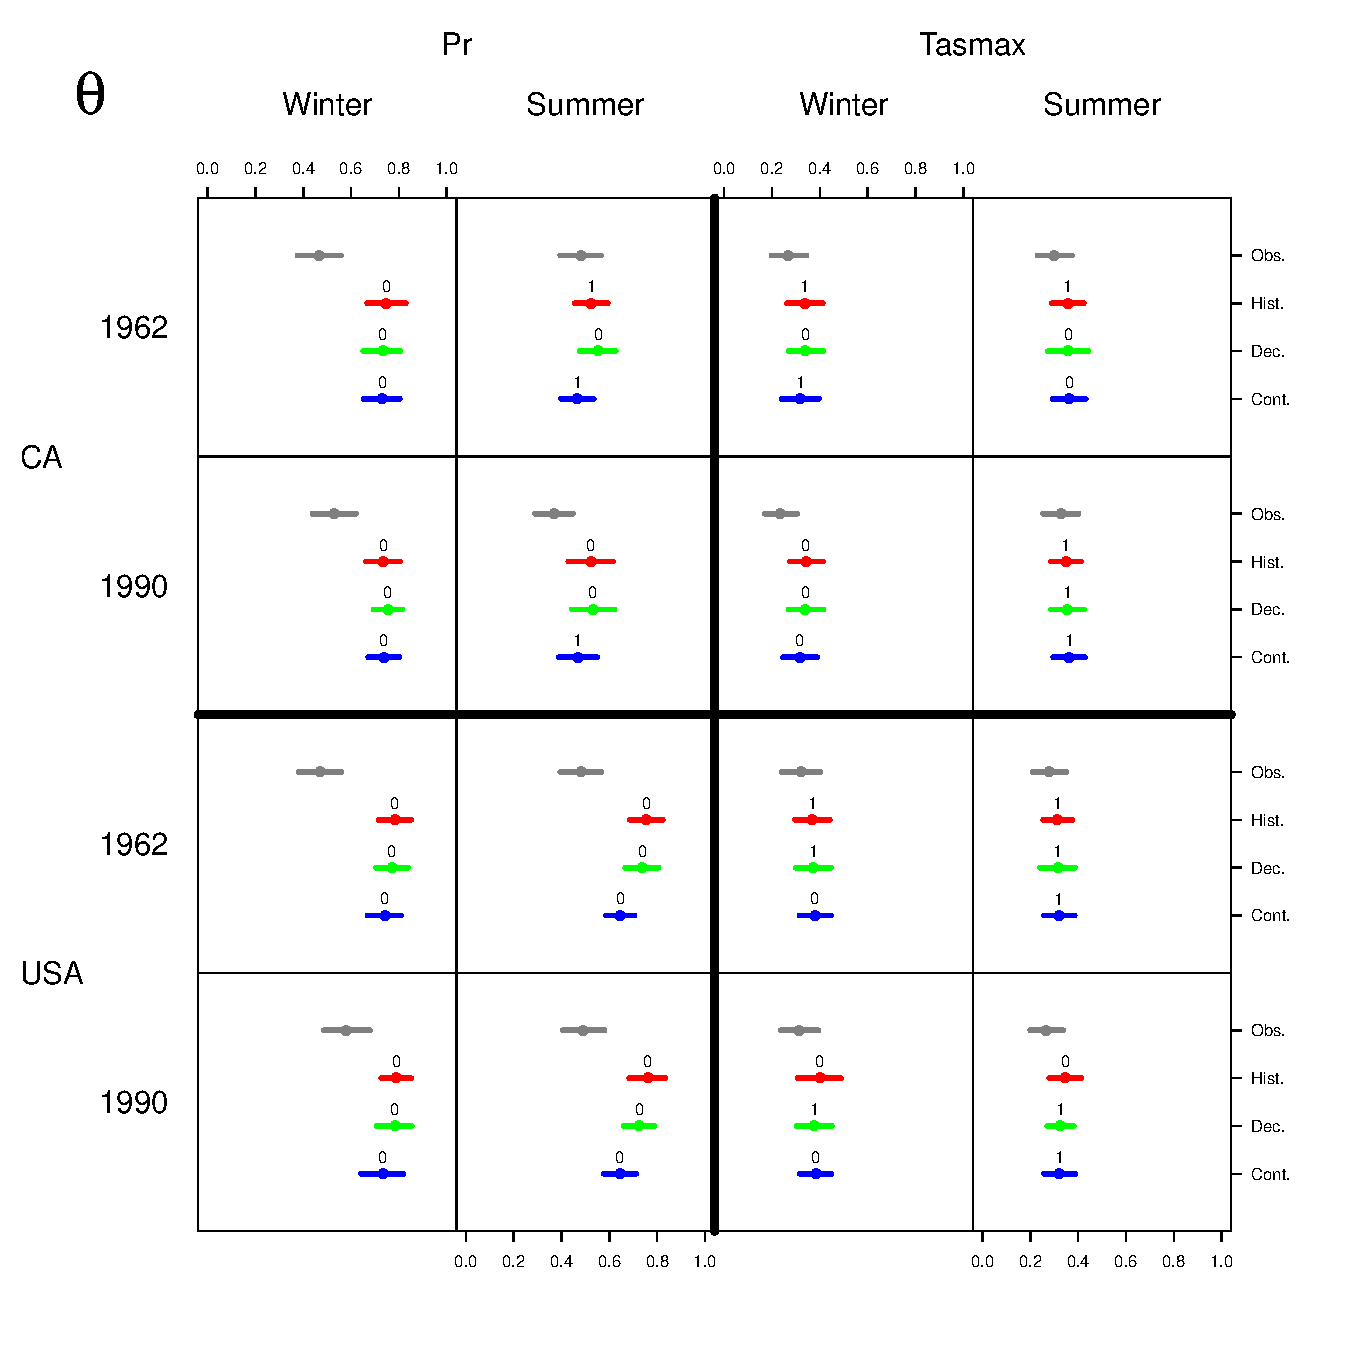
\includegraphics[scale=0.61]{figs/theta.pdf}
%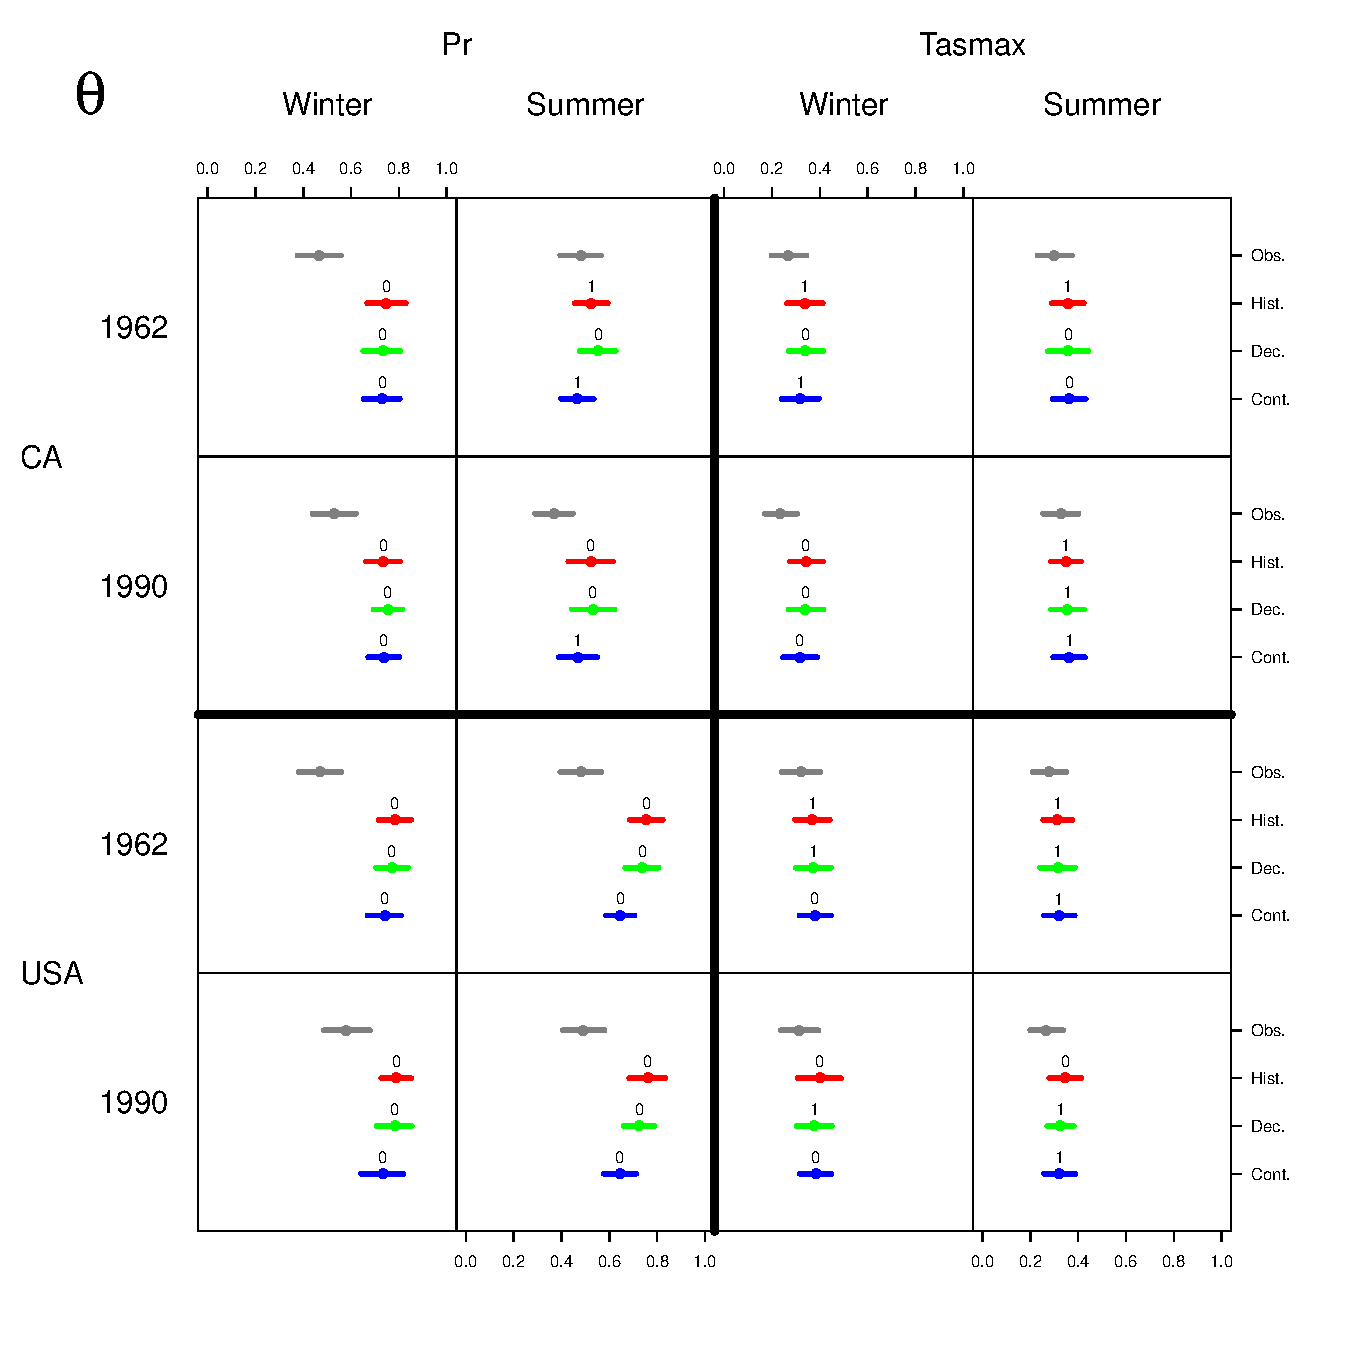
\includegraphics[scale=0.72]{figs/theta.pdf}
%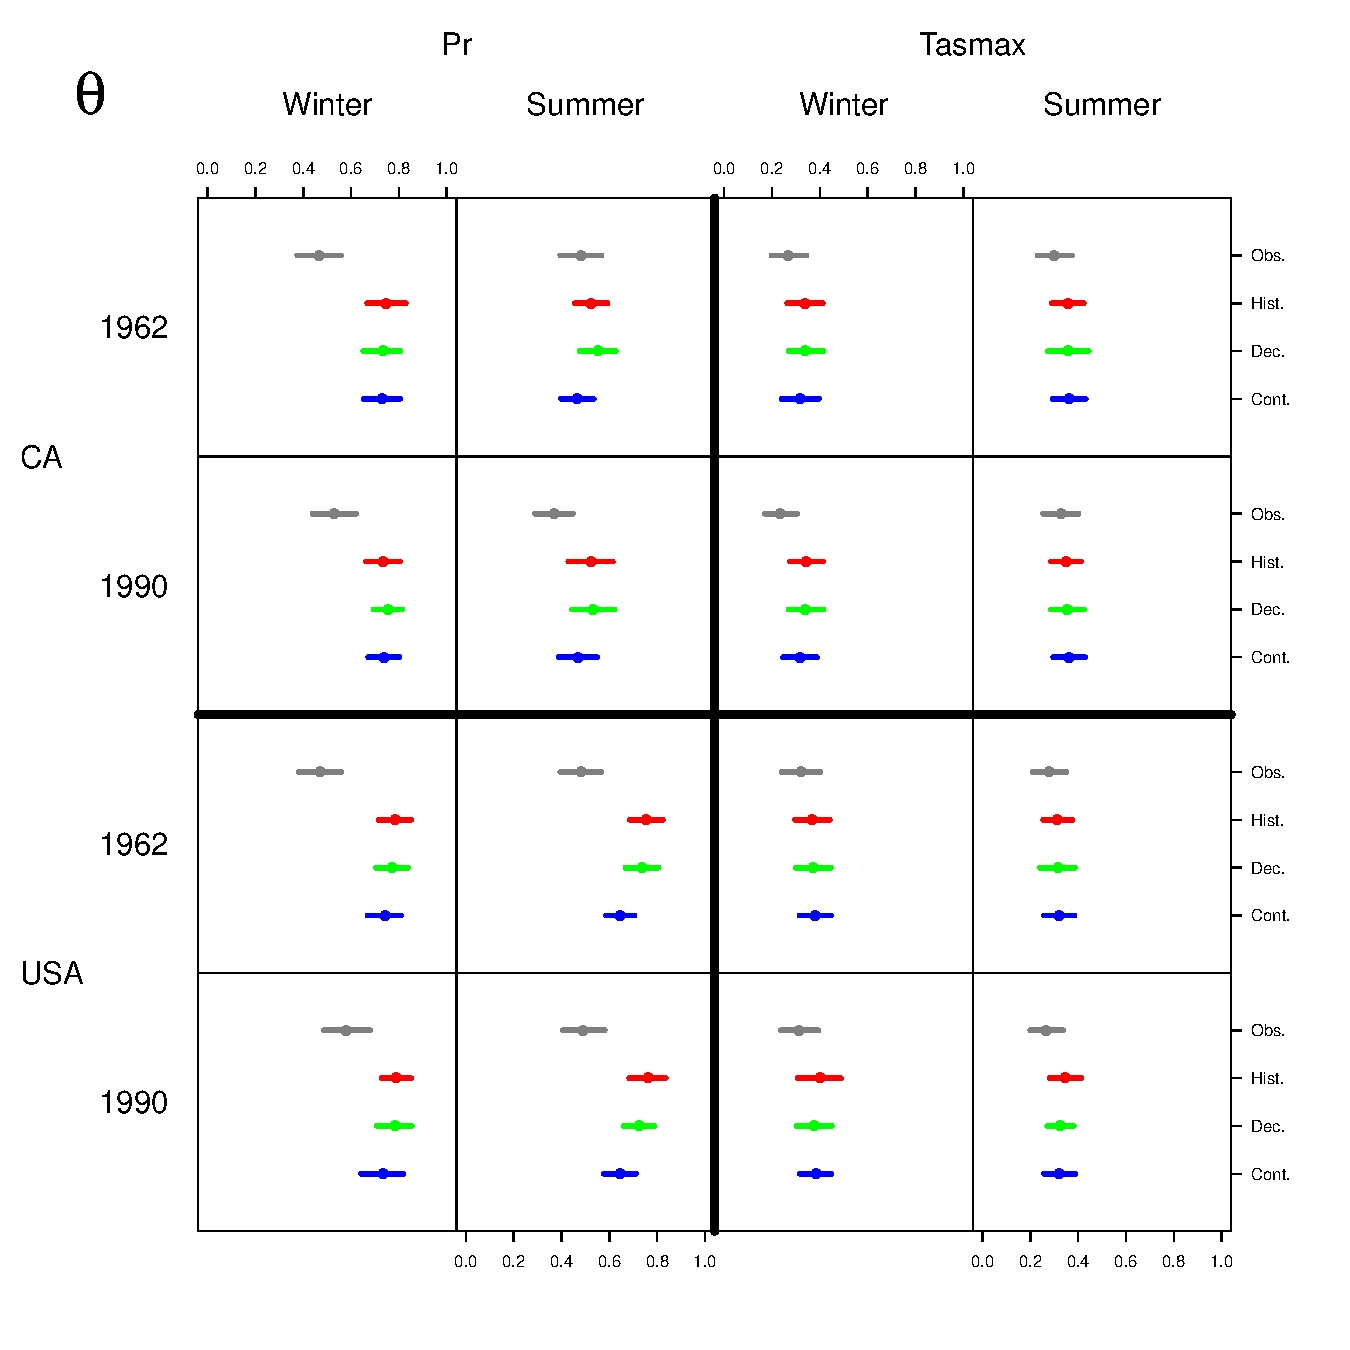
\includegraphics[scale=0.72]{figs/theta_nb.pdf}
\end{center}
\caption{The mean extremal index. Like the parameters shown in Figures \ref{ksi} and \ref{sigma}, the hierarchical mean is shown for the CanCM4 simulations.}
\label{theta}
\end{figure}

\begin{figure}
\begin{center}
 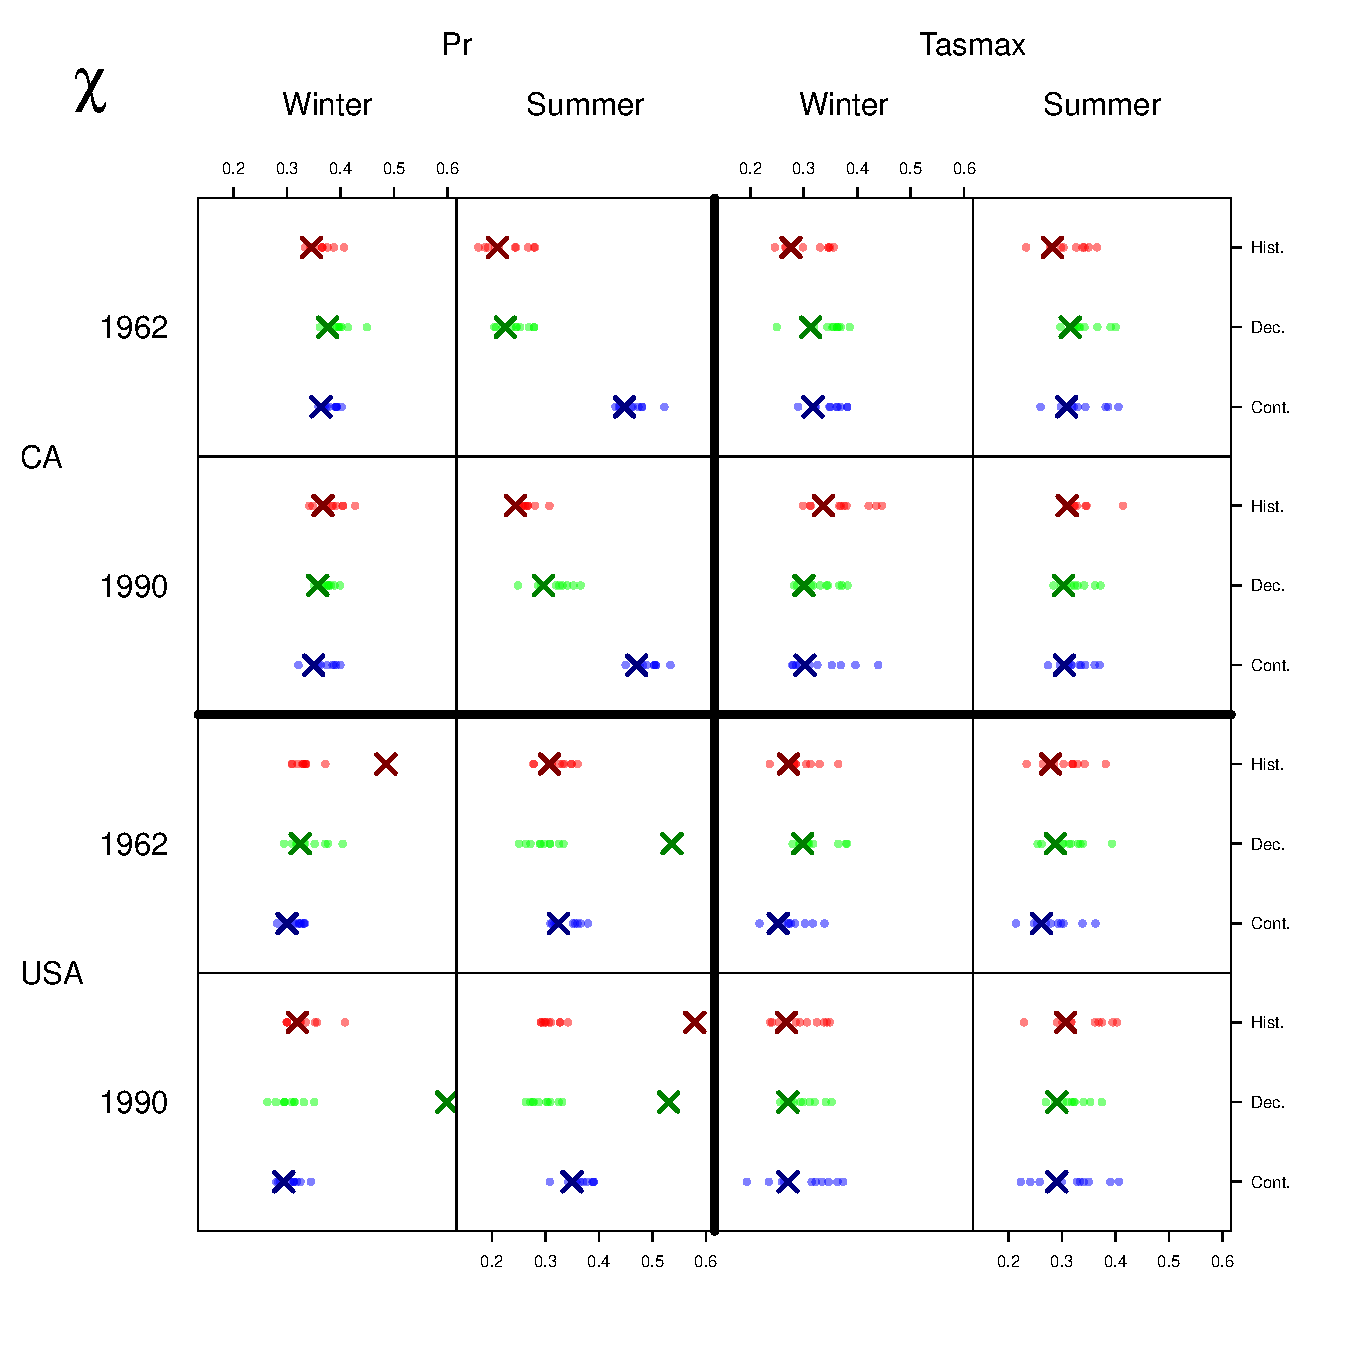
\includegraphics[scale=0.61]{figs/chi4.pdf}
%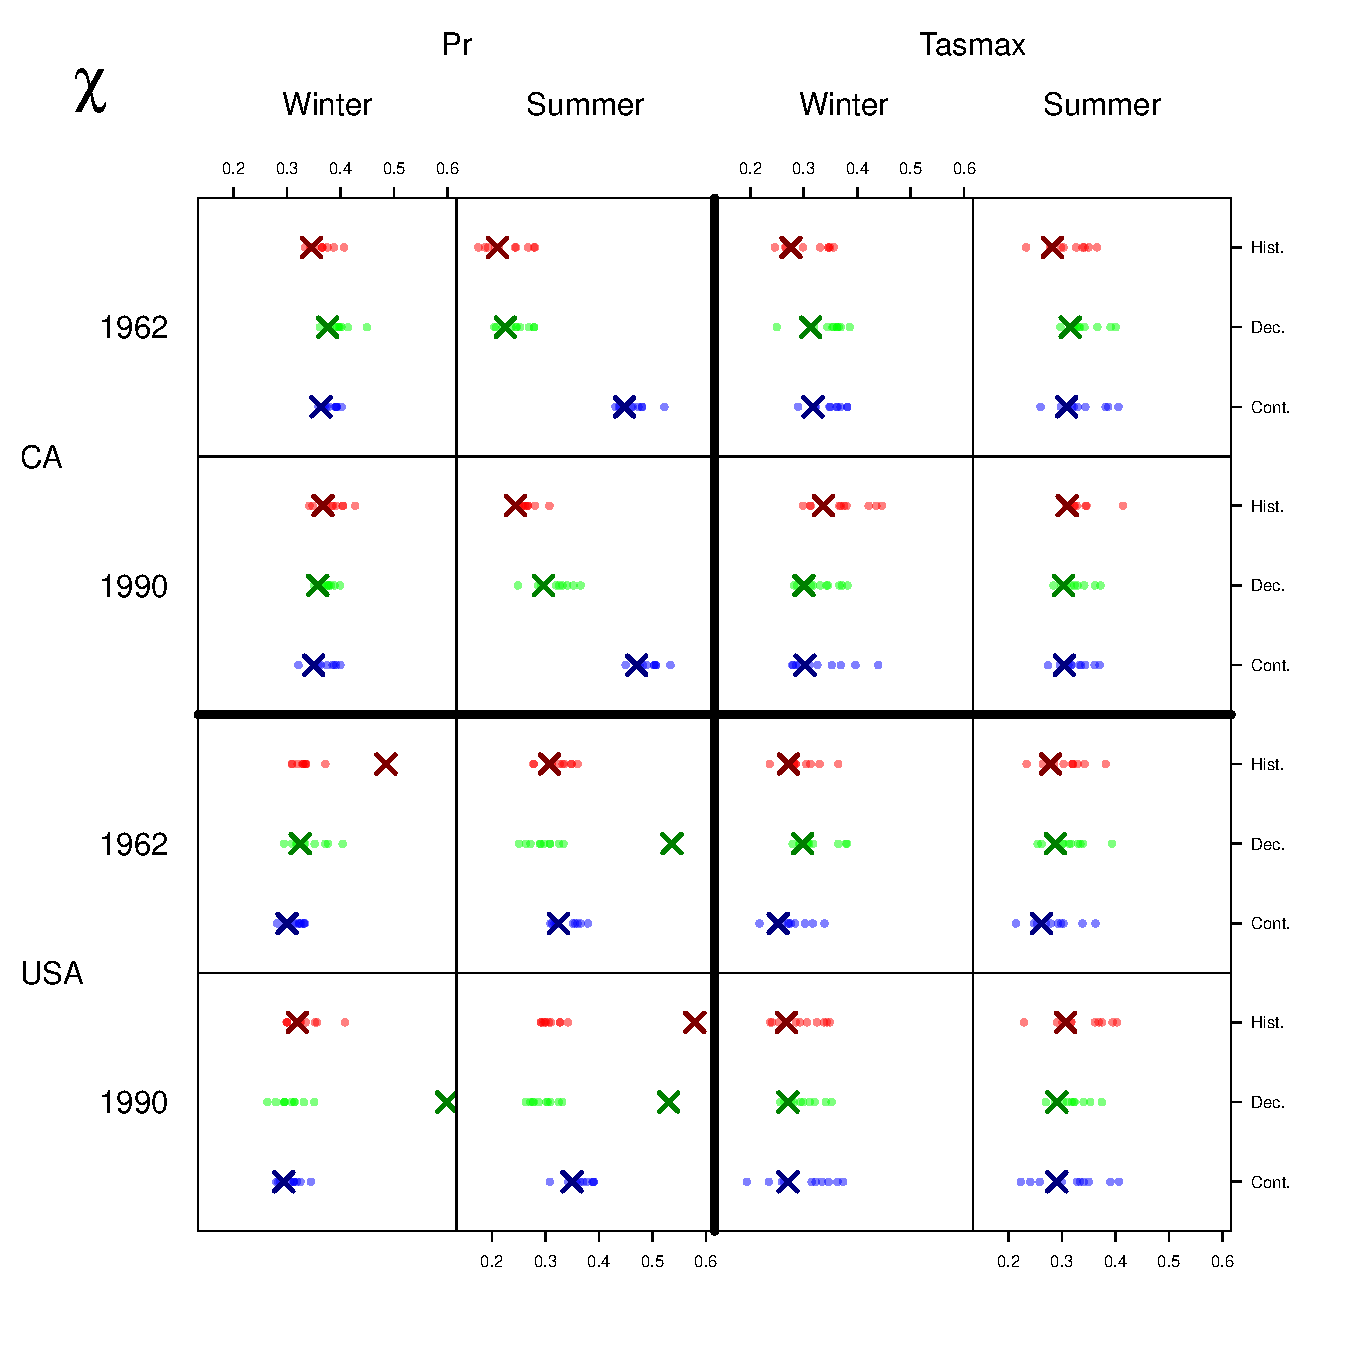
\includegraphics[scale=0.72]{figs/chi4.pdf}
\end{center}
\caption{Measure of asymptotic dependence, calculated using results from the simple Pareto process. The dots mark the $\chi$ for each replicate against the observations. The X marks the value of $\xi$ when all replicates are taken together.}
\label{chi}
\end{figure}


Figures \ref{ksi} through \ref{theta} show posterior parameters and other quantities of interest from the univariate analysis. For the hierarchical model, we show the results of the \emph{mean} process. For example, in Figure \ref{ksi} the parameter shown is the posterior for $\xi$, the mean of $\xi_1,\ldots,\xi_R$. This is in opposition to inference on an unknown replicate which would require sampling, among other things, a new shape parameter $\xi^*$. Therefore, the intervals are more narrow than if we looked at the posterior predictive distribution for a new replicate, but the parameters will be comparable to those from the univariate model with the observations and give us a sense of how the climate simulation performs on average.

The posterior shape parameters in Figure \ref{ksi} show overlapping bounds in many cases, but in some combinations of factors we can see some departure from the observations. The numbers shown above the lines are indicators for whether the posterior from the observations is similar to the posterior of the replicates---in the sense of Bhattacharyya distance described in section \ref{bhatta}---for a particular simulation class.
% TODO: find references for this claim, Weller et al. doesn't confirm it
% Perhaps an unexpected result is that, except for summer precipitation, there is evidence that total precipitation is bounded above (due to $\xi<0$). This is contrary to some findings that the shape parameter for precipitation is positive. [ADD REFS: This was mentioned a lot at SAMSI, so there should be some reference to it, right?]

Figure \ref{sigma} shows the logarithm of the mean scale parameter, $\log(\sigma)$ for the observations and $\log(\alpha/\beta)$ for the simulations, and the posteriors for $\zeta$, the probability of exceeding the threshold, are given in Figure \ref{zeta}.

Figures \ref{20rl} and \ref{50rl} give the $20$- and $50$-year return levels, respectively. In these figures, we have the same $x$-axes for the columns in total precipiation and for the columns under average maximum temperature. Some intervals are difficult to see given the scale, but we can still inspect how the return levels from the observations differ from those of the climate siulations. There is evidence of similarity between the data sources for maximum temperature (except for the 1962--1971 decade in the United States). The simulations struggle to find agreement with the observations when considering precipitation, only having two domains where the observations are similar to at least two of the climate sources (1990 USA Winter and 1962 USA Summer).

Figure \ref{tail} shows posterior predictive samples (based on the mean parameters for the hierarchical model) drawn from the generalized Pareto distribution, conditioned on the random variables being greater than the given threshold. With respect to the 95\% posterior intervals, there is significant overlap of the simulations with the observations, but this is not the case with Bhattacharyya distance. This is because nearly all replicates were very close to their mean, having a distance of roughly $0.02$, while the observations were different enough to have a distance of about $0.2$ from the mean process. Despite all this, we saw in Figures \ref{20rl} and \ref{50rl} that there is still some similarity between the important return level quantities, which account for $\zeta$ and $\theta$.

The posterior mean and 95\% highest posterior density intervals for the extremal index are shown in Figure \ref{theta}. The climate simulations seem to be consistent with the observations for the temperature, but not so for precipiation where they tend to overestimate $\theta$. The Bhattacharyya distance was not computed for these parameters.

Estimates for asymptotic dependence are given in Figure \ref{chi}. Many of them are in the region $[0.2, 0.4]$ indicating weak to moderate dependence. In only two instances do we have $\chi$ close to $0.5$. And in these cases the comparison is made with the control runs, which should be some cause of concern since the times for the control runs do not have the same meaning as those from the observations. In every other case we see relatively the same strength of dependence from the three climate simulations, though the dependence is weak.
